\title{Rokkoチュートリアル}

\newtheorem{rei}{例}
\renewcommand{\therei}{}
\newcommand{\smallscr}[1]{\scalebox{0.4}{$#1$}}
\newcommand{\middlescr}[1]{\scalebox{0.60}{$#1$}}
%\usepackage{multirow}

\newlength\savedwidth
\newcommand\whline{%
    \noalign{\xdef\origarrayrulewidth{\the\arrayrulewidth}%
    \global\arrayrulewidth 3\arrayrulewidth}%
    \hline%
    \noalign{\global\arrayrulewidth\origarrayrulewidth}%
}

\AtBeginSection[]{
    \begin{frame}
        \tableofcontents[currentsection]
    \end{frame}
}

\begin{document}

\lstset{language=c++,basicstyle=\ttfamily\tiny,showspaces=false,keepspaces=true,rulecolor=\color[cmyk]{0, 0.29,0.84,0}}

\begin{frame}
  \titlepage
  \noindent {\footnotesize 講習資料: \url{https://github.com/cmsi/rokko-tutorial/releases/latest}} 
\end{frame}

%% \section*{Outline}
%% \begin{frame}
%%   \tableofcontents
%% \end{frame}

\section{チュートリアルの概要}

\begin{frame}{Rokkoチュートリアル}
  \begin{itemize}
  \item 資料作成
    \setlength{\itemsep}{1em}
    \begin{itemize}
      \setlength{\itemsep}{1em}
    \item 坂下達哉 (東大物性研) \ \href{mailto:t-sakashita@issp.u-tokyo.ac.jp}{t-sakashita@issp.u-tokyo.ac.jp}
    \item 藤堂眞治 (東大院理/物性研) \ \href{mailto:wistaria@phys.s.u-tokyo.ac.jp}{wistaria@phys.s.u-tokyo.ac.jp}
    \end{itemize}
  \item 主催
    \begin{itemize}
    \item CMSI: 計算物質科学イニシアティブ \url{http://cms-initiative.jp/}
    \end{itemize}
  \end{itemize}
\end{frame}

\begin{frame}
  \frametitle{チュートリアルの流れ}
  \begin{itemize}
    %\setlength{\itemsep}{1em}
  \item 座学: 固有値問題の解法・固有値ソルバ/線形計算ライブラリ
  \item 座学: Rokkoの概要と内部構造
  \item 実習: Rokkoのインストール
  \item 座学・実習: 密行列向け逐次ソルバの基本概念、サンプル実行
  \item 座学・実習: 密行列向けMPI並列ソルバの基本概念、サンプル実行
  \item 座学・実習: 疎行列向けMPI並列ソルバの基本概念、サンプル実行
  \item 実習: 量子スピン系の対角化のサンプル実行
  %\item 実習: TITPACK2へのRokko組み込み実習
  \item 実習: アプリケーションからのRokkoの利用
%  \item (付録: ALPS/Baristaパッケージ)
 % \item (付録: MateriAppsとMateriApps LIVE!)
  \end{itemize}
\end{frame}


\section{固有値問題の解法・固有値ソルバ/線形計算ライブラリ}

\begin{frame}
  \frametitle{固有値問題の解法・固有値ソルバ/線形計算ライブラリ}
  \begin{itemize}
    \setlength{\itemsep}{1em}
  \item 行列の対角化
  \item 固有値問題の解法
  \item 固有値ソルバ/線形計算ライブラリ
  \end{itemize}
\end{frame}

\begin{frame}
  \frametitle{行列の対角化}
  \begin{itemize}
    %\setlength{\itemsep}{1em}
  \item 行列の種類
    \begin{itemize}
    \item 実対称行列, 実非対称行列, エルミート行列, 非エルミート行列
    \end{itemize}
  \item 行列の表示
    \begin{itemize}
      \item 密行列, CRS(Compressed Row Storage)形式, MatFree形式\\
            (それぞれTITPACK2の「小規模」, 「中規模」, 「大規模」に対応)
    \end{itemize}
  \item 必要な固有値
    \begin{itemize}
      \item 全て, 絶対値の大きな(小さな)順にいくつか, ある範囲内
    \end{itemize}
  \item 固有ベクトル
    \begin{itemize}
      \item 要/不要
    \end{itemize}
  \end{itemize}
\end{frame}

\begin{frame}
  \frametitle{用語の定義}
  \begin{itemize}
    %\setlength{\itemsep}{1em}
  \item 固有値問題の解法(Eigenvalue algorithm)
    \begin{itemize}
      \item 固有値問題を解くためのアルゴリズム
    \end{itemize}
  \item 固有値ソルバ(Eigensolver, Eigenvalue problem solver)
    \begin{itemize}
      \item 固有値解法の実装
    \end{itemize}
  \item 固有値ソルバライブラリ(Eigensolver Library)
    \begin{itemize}
      \item 固有値ソルバのみを含むライブラリ
    \end{itemize}
  \item 線形計算ライブラリ(Linear Algebra Library)
    \begin{itemize}
      \item 固有値ソルバや他の線形計算ソルバの集合体
    \end{itemize}
  \item 厳密対角化パッケージ(Exact diagonalization package)
    \begin{itemize}
      \item 量子格子模型のハミルトニアンの固有値問題を扱うソフトウェア
    \end{itemize}
  \end{itemize}
\end{frame}

\begin{frame}
  \frametitle{固有値問題の解法(一部)}
  \begin{itemize}
    %\setlength{\itemsep}{1em}
  \item 三重対角行列に対する固有値問題の解法
    \begin{itemize}
      \item 二分法, QR法, MR3, 分割統治法+QR法
    \end{itemize}
  \item 密行列の直接対角化
    \begin{itemize}
      \item Jacobi法
    \end{itemize}
  \item 密行列の三重対角化
    \begin{itemize}
      \item Householder法
    \end{itemize}
  \item 疎行列の直接対角化
    \begin{itemize}
      \item べき乗法, 逆べき乗法, レイリー商反復法, Jacobi-Davidson法, LOBPCG, Krylov-Schur法
    \end{itemize}
  \item 疎行列の三重対角化
    \begin{itemize}
      \item Lanczos法, Arnoldi法, リスタート付きLanczos法(Restart Lanczos), Thick-restart Lanczos法
    \end{itemize}
  \item その他の方法
    \begin{itemize}
      \item Sakurai-Sugiura法
    \end{itemize}
  \end{itemize}
\end{frame}

\begin{frame}
  \frametitle{固有値問題の解法}
  \begin{center}
    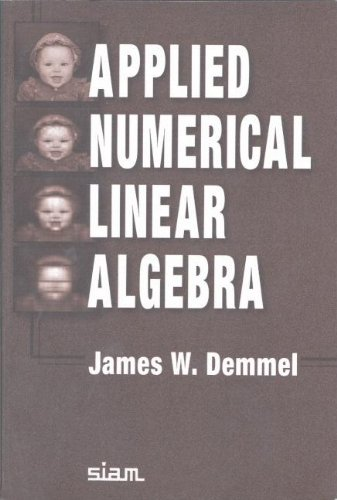
\includegraphics[height=0.45\textheight]{figure/AppliedNumericalLinearAlgebra.jpg} \ \
    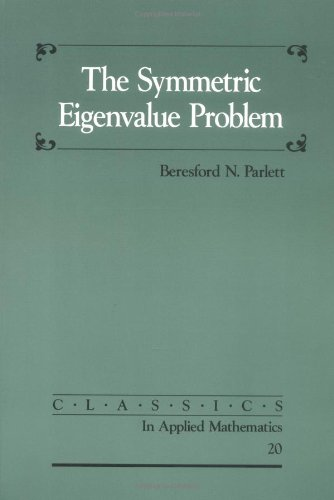
\includegraphics[height=0.45\textheight]{figure/TheSymmetricEigenvalueProblem.jpg} \ \
    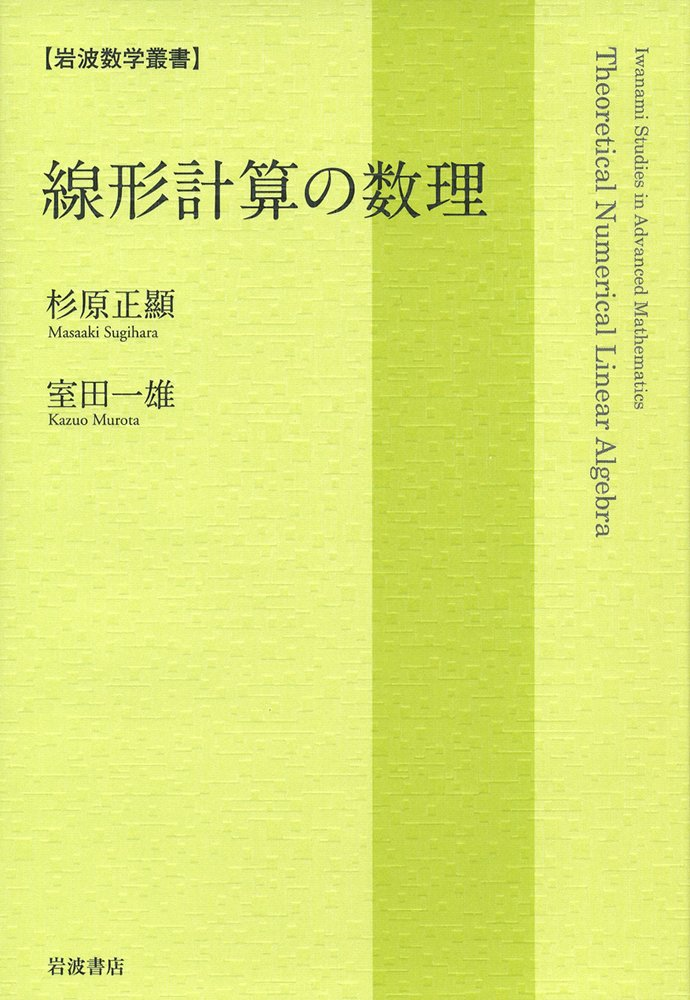
\includegraphics[height=0.45\textheight]{figure/SenkeikeisanNoSuri.jpg}  \ \
    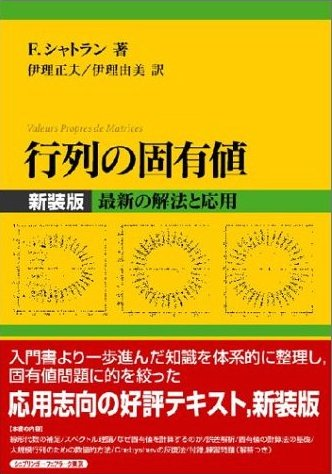
\includegraphics[height=0.45\textheight]{figure/GyoretsuNoKoyuchi.jpg}
  \end{center}
\end{frame}

\begin{frame}
  \frametitle{固有値ソルバライブラリ(密行列向け)}
  \begin{itemize}
    %\setlength{\itemsep}{1em}
  \item \href{http://www.aics.riken.jp/labs/lpnctrt/EigenExa.html}{EigenExa}: 密行列ソルバ
    \begin{itemize}
      \item Householder (3重対角化, 5重対角化)+分割統治法+QR
    \end{itemize}
  \item \href{http://elpa.rzg.mpg.de}{ELPA}
    \begin{itemize}
      \item Householder+分割統治法+QR
    \end{itemize}
  \end{itemize}
\end{frame}

\begin{frame}
  \frametitle{固有値ソルバライブラリ(疎行列向け)}
  \begin{itemize}
  \item \href{http://trilinos.org/packages/anasazi/}{Anasazi}: 反復法ソルバ中心
    \begin{itemize}
      \item Krylov-Schur, Jacobi-Davidson, XXX-Davidson, LOBPCG, Implicit Riemannian Trust Region Method
    \end{itemize}
  \item \href{http://www.caam.rice.edu/software/ARPACK/}{ARPACK}
    \begin{itemize}
      \item Implicit Restarted Lanczos
    \end{itemize}
  \item \href{https://code.google.com/p/blopex/}{BLOPEX}
    \begin{itemize}
    \item Locally Optimal Block Preconditioned Conjugate Gradient Method (LOBPCG)
    \end{itemize}
  \item \href{http://www.grycap.upv.es/slepc/}{SLEPc}: 反復法ソルバ中心, ビルド時に逐次かMPI並列かを選ぶ必要あり
    \begin{itemize}
      \item Krylov-Schur, Generalized Davidson, Jacobi-Davidson, Rayleigh Quotient Conjugate Gradient, Contour integral Sakurai-Sugiura, Power method, Subspace Itertation, Arnoldi (explicit restart), Lanczos (explicit restart) \\
    \end{itemize}
  \item \href{http://www.comp-phys.org/software/ietl/}{IETL}: ALPSに含まれる反復法ソルバ
    \begin{itemize}
      \item Lanczos, 他
    \end{itemize}
  \end{itemize}
\end{frame}

\begin{frame}
  \frametitle{線形計算ライブラリ(密行列向け)}
  \begin{itemize}
    %\setlength{\itemsep}{1em}
  \item LAPACK, ScaLAPACKのベンダ実装
    \begin{itemize}
    \item \href{https://developer.apple.com/library/mac/documentation/Accelerate/Reference/AccelerateFWRef/index.html}{Apple Accelerate Framework(BLAS/vecLib)}: LAPACK
    \item Fujitsu SSLII: LAPACK, ScaLAPACK(の一部), 他
    \item \href{https://software.intel.com/en-us/mkl_11.1_ref}{Intel MKL}: LAPACK, ScaLAPACK
    \item
      \href{http://developer.amd.com/tools-and-sdks/cpu-development/amd-core-math-library-acml/}{ACML(AMD
        Core Math Library)}: LAPACK
    \item \href{http://www.openblas.net}{OpenBLAS}: BLAS+一部の
      LAPACK(GotoBLASの後継)

    \end{itemize}
  \item \href{http://www.netlib.org/lapack/}{Netlib LAPACK}: LAPACKのリファレンス実装
    \begin{itemize}
      \item Householder+QR, Householder+分割統治法+QR, Householder+二分法, Householder+MR3
    \end{itemize}
  \item \href{http://www.netlib.org/scalapack/}{Netlib ScaLAPACK}: ScaLAPACKのリファレンス実装
    \begin{itemize}
      \item Householder+QR, Householder+分割統治法+QR, Householder+二分法, Householder+MR3
    \end{itemize}
  \item \href{http://eigen.tuxfamily.org/}{Eigen3}(逐次版、行列・行列積のみスレッド並列化)
    \begin{itemize}
      \item Householder+QR
    \end{itemize}
  \item \href{http://libelemental.org}{Elemental}:含まれる固有値ソルバMRRRは、プロセス数が平方数の場合のみ確実に動く
    \begin{itemize}
      \item Householder+MR3
    \end{itemize}
  \end{itemize}
\end{frame}

\begin{frame}
  \frametitle{線形計算ライブラリ(疎行列向け)}
  \begin{itemize}
    %\setlength{\itemsep}{1em}
  \item \href{http://trilinos.org}{Trilinos}:固有値ソルバライブラリAnasaziを含む
  \item Xabclib (\href{http://ppopenhpc.cc.u-tokyo.ac.jp/}{ppOpen AT})
  \end{itemize}
\end{frame}

\begin{frame}
  \frametitle{おすすめ順}
  \begin{itemize}
    %\setlength{\itemsep}{1em}
  \item 密行列・逐次
    \begin{itemize}
      \item LAPACK (のベンダ実装) $>$ Eigen3
    \end{itemize}
  \item 密行列・MPI並列
    \begin{itemize}
      \item EigenExa $>$ ELPA $>$ ScaLAPACK (のベンダ実装) $>$ Elemental
    \end{itemize}
  \item 疎行列(逐次、MPI並列)
    \begin{itemize}
      \item Anasazi $>$ SLEPc
    \end{itemize}
  \end{itemize}
\end{frame}

\begin{frame}{EigenExaによる超巨大密行列の対角化}
  \begin{center}
    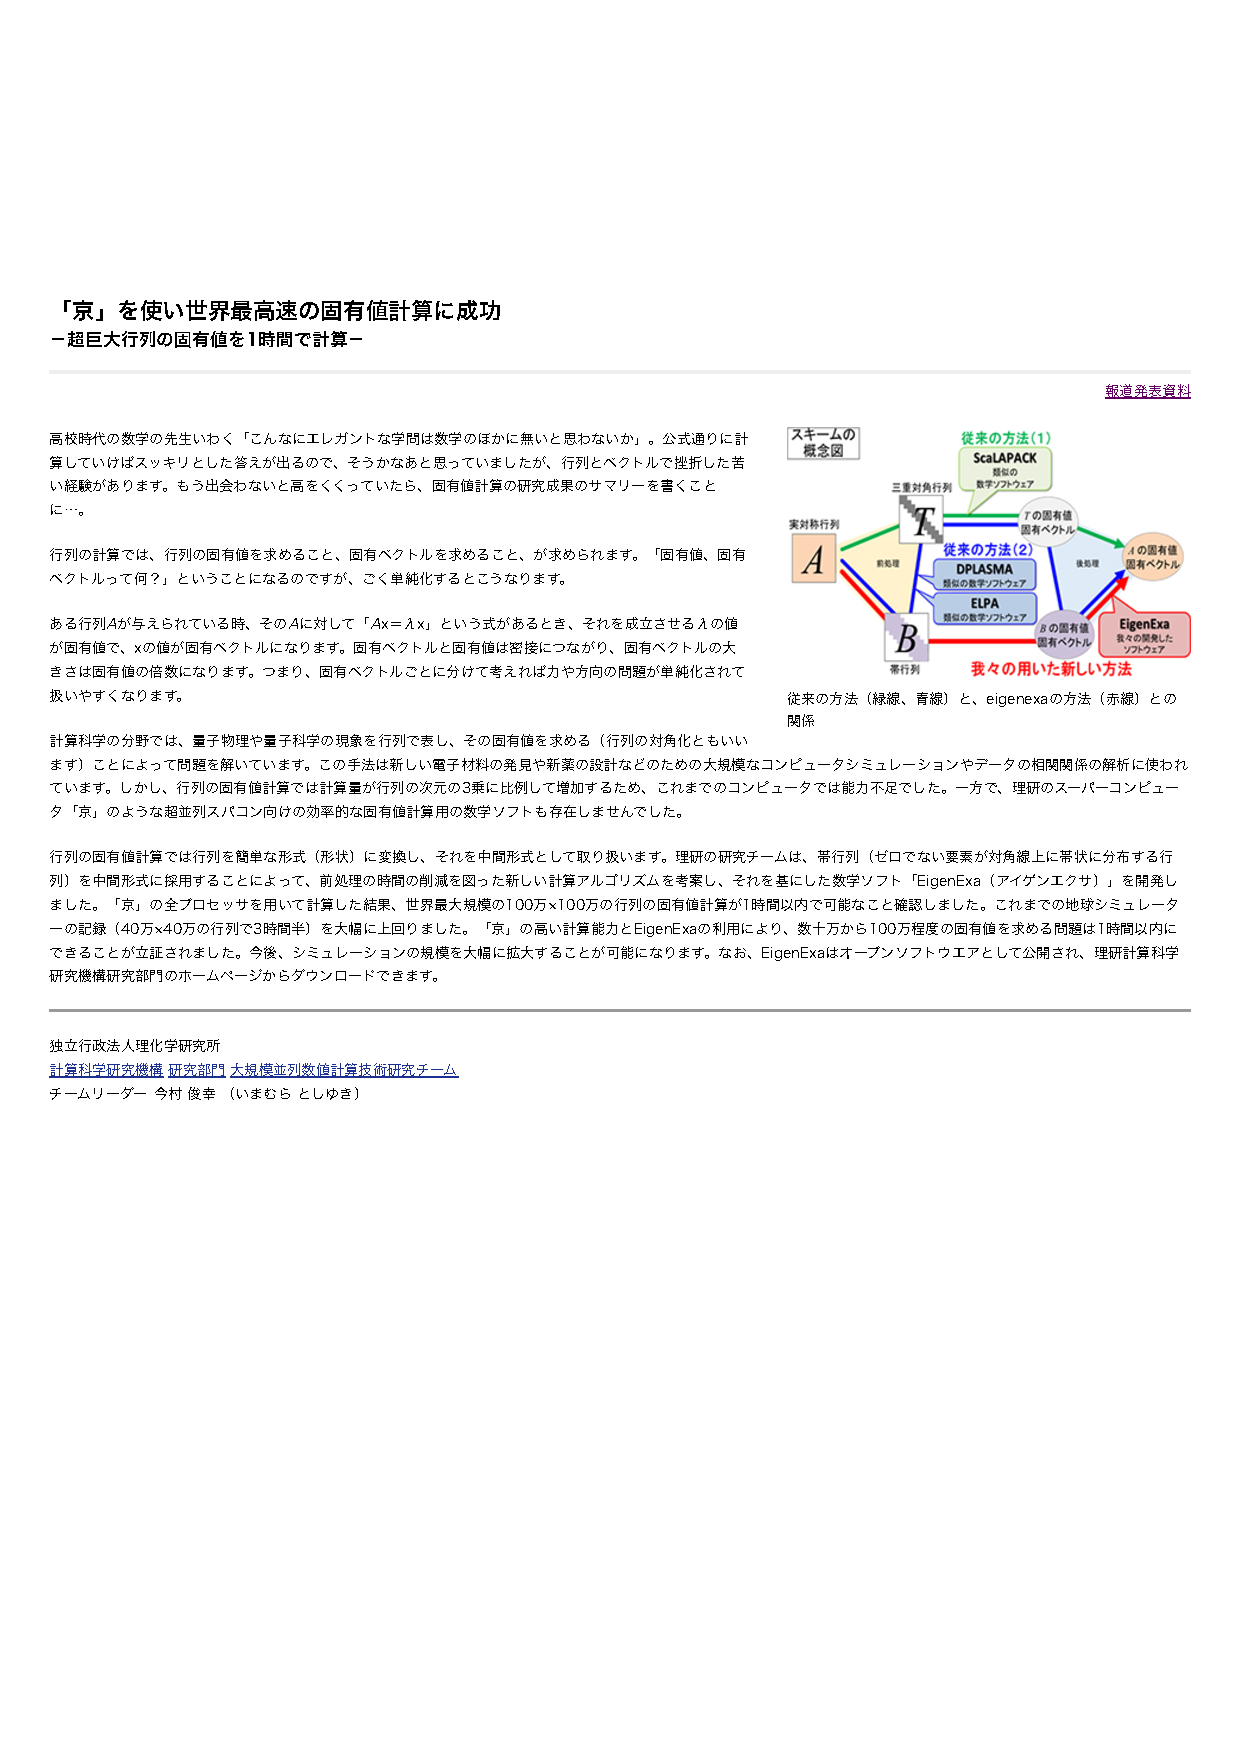
\includegraphics[height=0.8\textheight]{figure/eigenexa.pdf}
  \end{center}
\end{frame}

\begin{frame}
  \frametitle{最新の固有値ソルバ}
  \begin{itemize}
    \setlength{\itemsep}{1em}
  \item ハイブリッド並列(MPI+OpenMP)対応のソルバも増えてきた
  \item 超並列環境に対応した並列ソルバをユーザ自身が実装・最適化するの
    はもはや不可能
  \item 最新の並列固有値ソルバを積極的に活用すべき
  \end{itemize}
\end{frame}

\begin{frame}
  \frametitle{厳密対角化パッケージの状況}
  \begin{itemize}
    \setlength{\itemsep}{1em}
  \item 代表的なパッケージ
    \begin{itemize}
    \item ALPS (\href{http://alps.comp-phys.org/static/software/applications/diag/fulldiag/doc/}{fulldiag} / \href{http://alps.comp-phys.org/mediawiki/index.php/Documentation:sparsediag}{sparsediag}): LAPACK, IETLを利用
    \item \href{http://quattro.phys.sci.kobe-u.ac.jp/Kobe_Pack/Kobe_Pack.html}{KOBEPACK}: 独自の固有値ソルバを実装
    \item \href{http://www-e.uni-magdeburg.de/jschulen/spin/}{SPINPACK}: LAPACKを利用
    \item \href{http://www.noc.titech.ac.jp/~phys0016_nishimori/titpack2_new/index-e.html}{TITPACK2}: 独自の固有値ソルバを実装
    \end{itemize}
  \item 逐次 or スレッド並列のみ, MPI並列なし
  \item 最新の超並列スパコン環境を活かしきれていない
  \end{itemize}
\end{frame}

\begin{frame}
  \frametitle{固有値解法とソルバ}
  \begin{itemize}
    \setlength{\itemsep}{1em}
    \item GitHub Wikiに, 固有値問題の解法, 固有値ソルバ, 固有値ソルバ/線形計算ライブラリ, 厳密対角化パッケージに関するリファレンス・マニュアルを作成中
      \begin{itemize}
        \item 固有値解法とソルバ: \url{https://github.com/t-sakashita/rokko/wiki/EigenvalueAlgorithms}
      \end{itemize}
    \item ボランティア募集中!
  \end{itemize}
\end{frame}
        
\section{Rokkoの概要と内部構造}

\begin{frame}
  \frametitle{Rokkoの概要と内部構造}
  \begin{itemize}
    \setlength{\itemsep}{1em}
  \item 既存のライブラリの問題点
  \item Rokkoの概要
  \item 並列ソルバの基本概念
  \item Rokkoの内部構造
  \end{itemize}
\end{frame}

\begin{frame}
  \frametitle{既存のライブラリの問題点}
  \begin{itemize}
    \setlength{\itemsep}{1em}
  \item ソルバ毎に異なるデザイン
  \item インストール方法もライブラリ毎に異なる
  \item ドキュメントが不十分な場合も多い
  \item コンピュータのアーキテクチャ毎に異なるコンパイル・リンクオプションが必要
  \item C++/C/Fortran相互リンクの問題
  \item ライブラリ間の依存関係が複雑
  \item 実際に試す前に大まかな性能比較が欲しい
  \end{itemize}
\end{frame}

\begin{frame}
  \frametitle{ライブラリ間の依存関係(密行列向け)}
  \begin{center}
    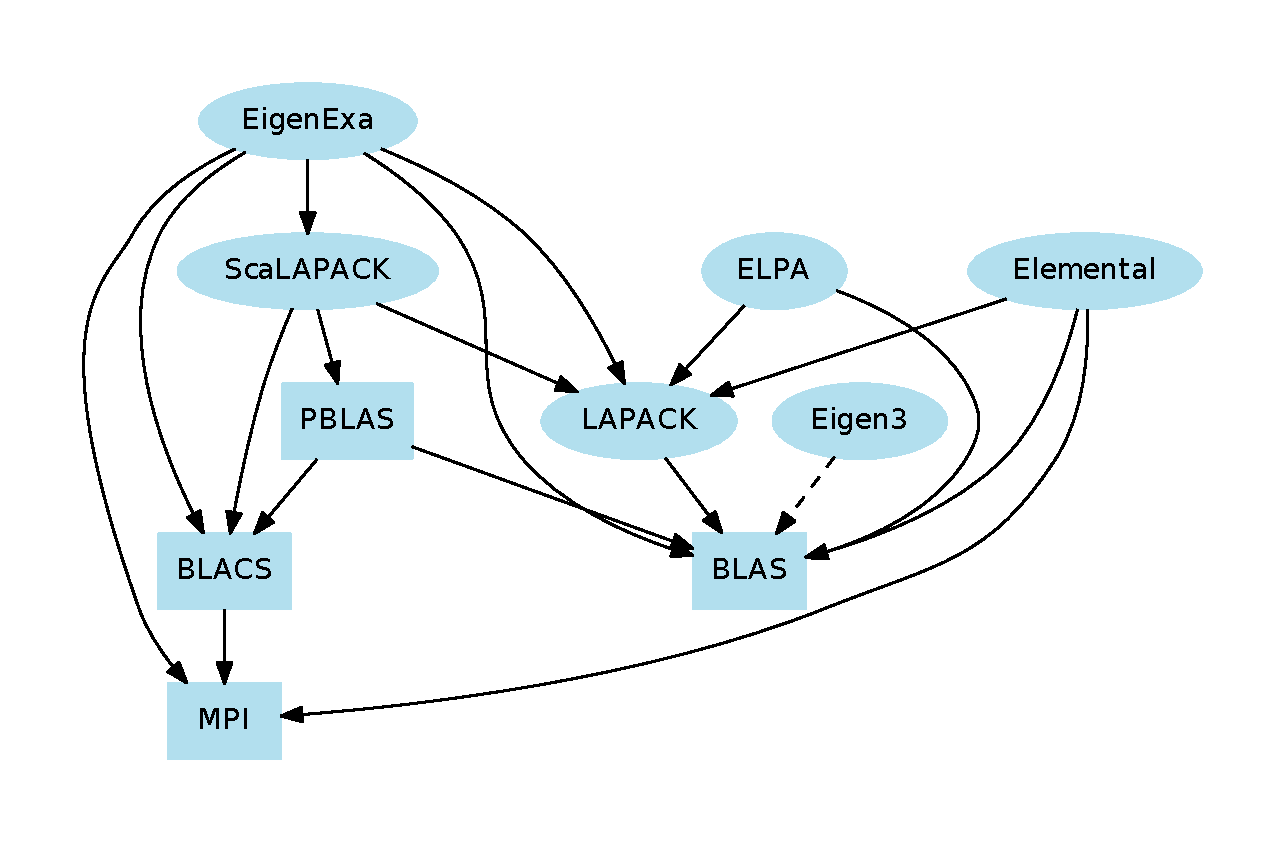
\includegraphics[height=0.8\textheight]{figure/eigensolver_dependency.pdf}
  \end{center}
\end{frame}

\begin{frame}
  \frametitle{Rokkoの開発者}
  \begin{itemize}
    \setlength{\itemsep}{1em}
  \item 坂下達哉 (東大物性研) \ \href{mailto:t-sakashita@issp.u-tokyo.ac.jp}{t-sakashita@issp.u-tokyo.ac.jp}
  \item 五十嵐 亮 (東大物性研) \ \href{mailto:rigarash@issp.u-tokyo.ac.jp}{rigarash@issp.u-tokyo.ac.jp}
  \item 本山裕一 (東大物性研) \ \href{mailto:y-motoyama@issp.u-tokyo.ac.jp}{y-motoyama@issp.u-tokyo.ac.jp}
  \item 大久保 毅 (東大物性研) \ \href{mailto:t-okubo@issp.u-tokyo.ac.jp}{t-okubo@issp.u-tokyo.ac.jp}
  \item 藤堂眞治 (東大院理/物性研) \ \href{mailto:wistaria@phys.s.u-tokyo.ac.jp}{wistaria@phys.s.u-tokyo.ac.jp}
  \end{itemize}
\end{frame}

\begin{frame}
  \frametitle{Rokkoの概要}
  \begin{itemize}
    %\setlength{\itemsep}{1em}
  \item 使用言語
    \begin{itemize}
      %\setlength{\itemsep}{1em}
    \item コア部分: C++
    \item 言語バインディング: C, Fortran90
    \item ベンチマークスクリプト: Python
    \end{itemize}
  \item ライセンス
    \begin{itemize}
      %\setlength{\itemsep}{1em}
    \item Boostライセンス (ほぼ自由に使える)
    \end{itemize}
  \item ソースコード
    \begin{itemize}
      %\setlength{\itemsep}{1em}
    \item GitHubで公開\\
          \url{https://github.com/t-sakashita/rokko/}
    \end{itemize}
  \end{itemize}
\end{frame}

\begin{frame}
  \frametitle{VCS (Version Control System)によるソース管理}
  \begin{itemize}
  \item 開発者が複数になると, ディレクトリ名やログファイルによるバージョン管理はすぐに破綻する
  \item ソースコードをサーバー上で一括管理
    \begin{itemize}
    \item ネットワーク経由でソースを check out/check in
    \end{itemize}
  \item 全ての修正履歴を保存
  \item 複数人が同時に更新した場合に衝突を回避するしくみ
  \item ブランチ・マージ・タグ付けなどが可能
  \item 開発者が一人, 公開の予定がない場合でも積極的に使うべき
  \item 参考資料: バージョン管理web講習会 {\tiny
      \url{http://www.cms-initiative.jp/ja/research-support/develop-support/how-to-publish/develop-apps/dt0l33}}
  \end{itemize}
\end{frame}

\begin{frame}
  \frametitle{Rokkoの設計方針}
  \begin{itemize}
    \setlength{\itemsep}{1em}
  \item 共通のベクトルや行列クラス
  \item ソルバの違いはラッパーで吸収
    \begin{itemize}
      %\setlength{\itemsep}{1em}
    \item 個々のソルバに仕様変更があってもRokkoが吸収
    \end{itemize}
  \item 再コンパイルなしに, 実行時にソルバを選択可能
  \item 仮想関数とテンプレートを組み合わせることで, オーバーヘッドの少ないラッパーを実装
  \item C++, C, Fortran90から使用可能に
  \end{itemize}
\end{frame}

\begin{frame}
  \frametitle{Rokkoの全体像}
  \begin{itemize}
    %\setlength{\itemsep}{1em}
  \item 固有値ソルバ/線形演算ライブラリのインストールスクリプト
  \item 共通基本クラス(分散行列, プロセスグリッド他)
  \item 固有値ソルバラッパー(C++)
  \item 固有値ソルバ・ファクトリ(C++)
  \item C/Fortranラッパー
  \item テスト・サンプルプログラム
  \item ベンチマークスクリプト
  \end{itemize}
\end{frame}

\begin{frame}
  \frametitle{Rokko Software Stack}
  \begin{center}
    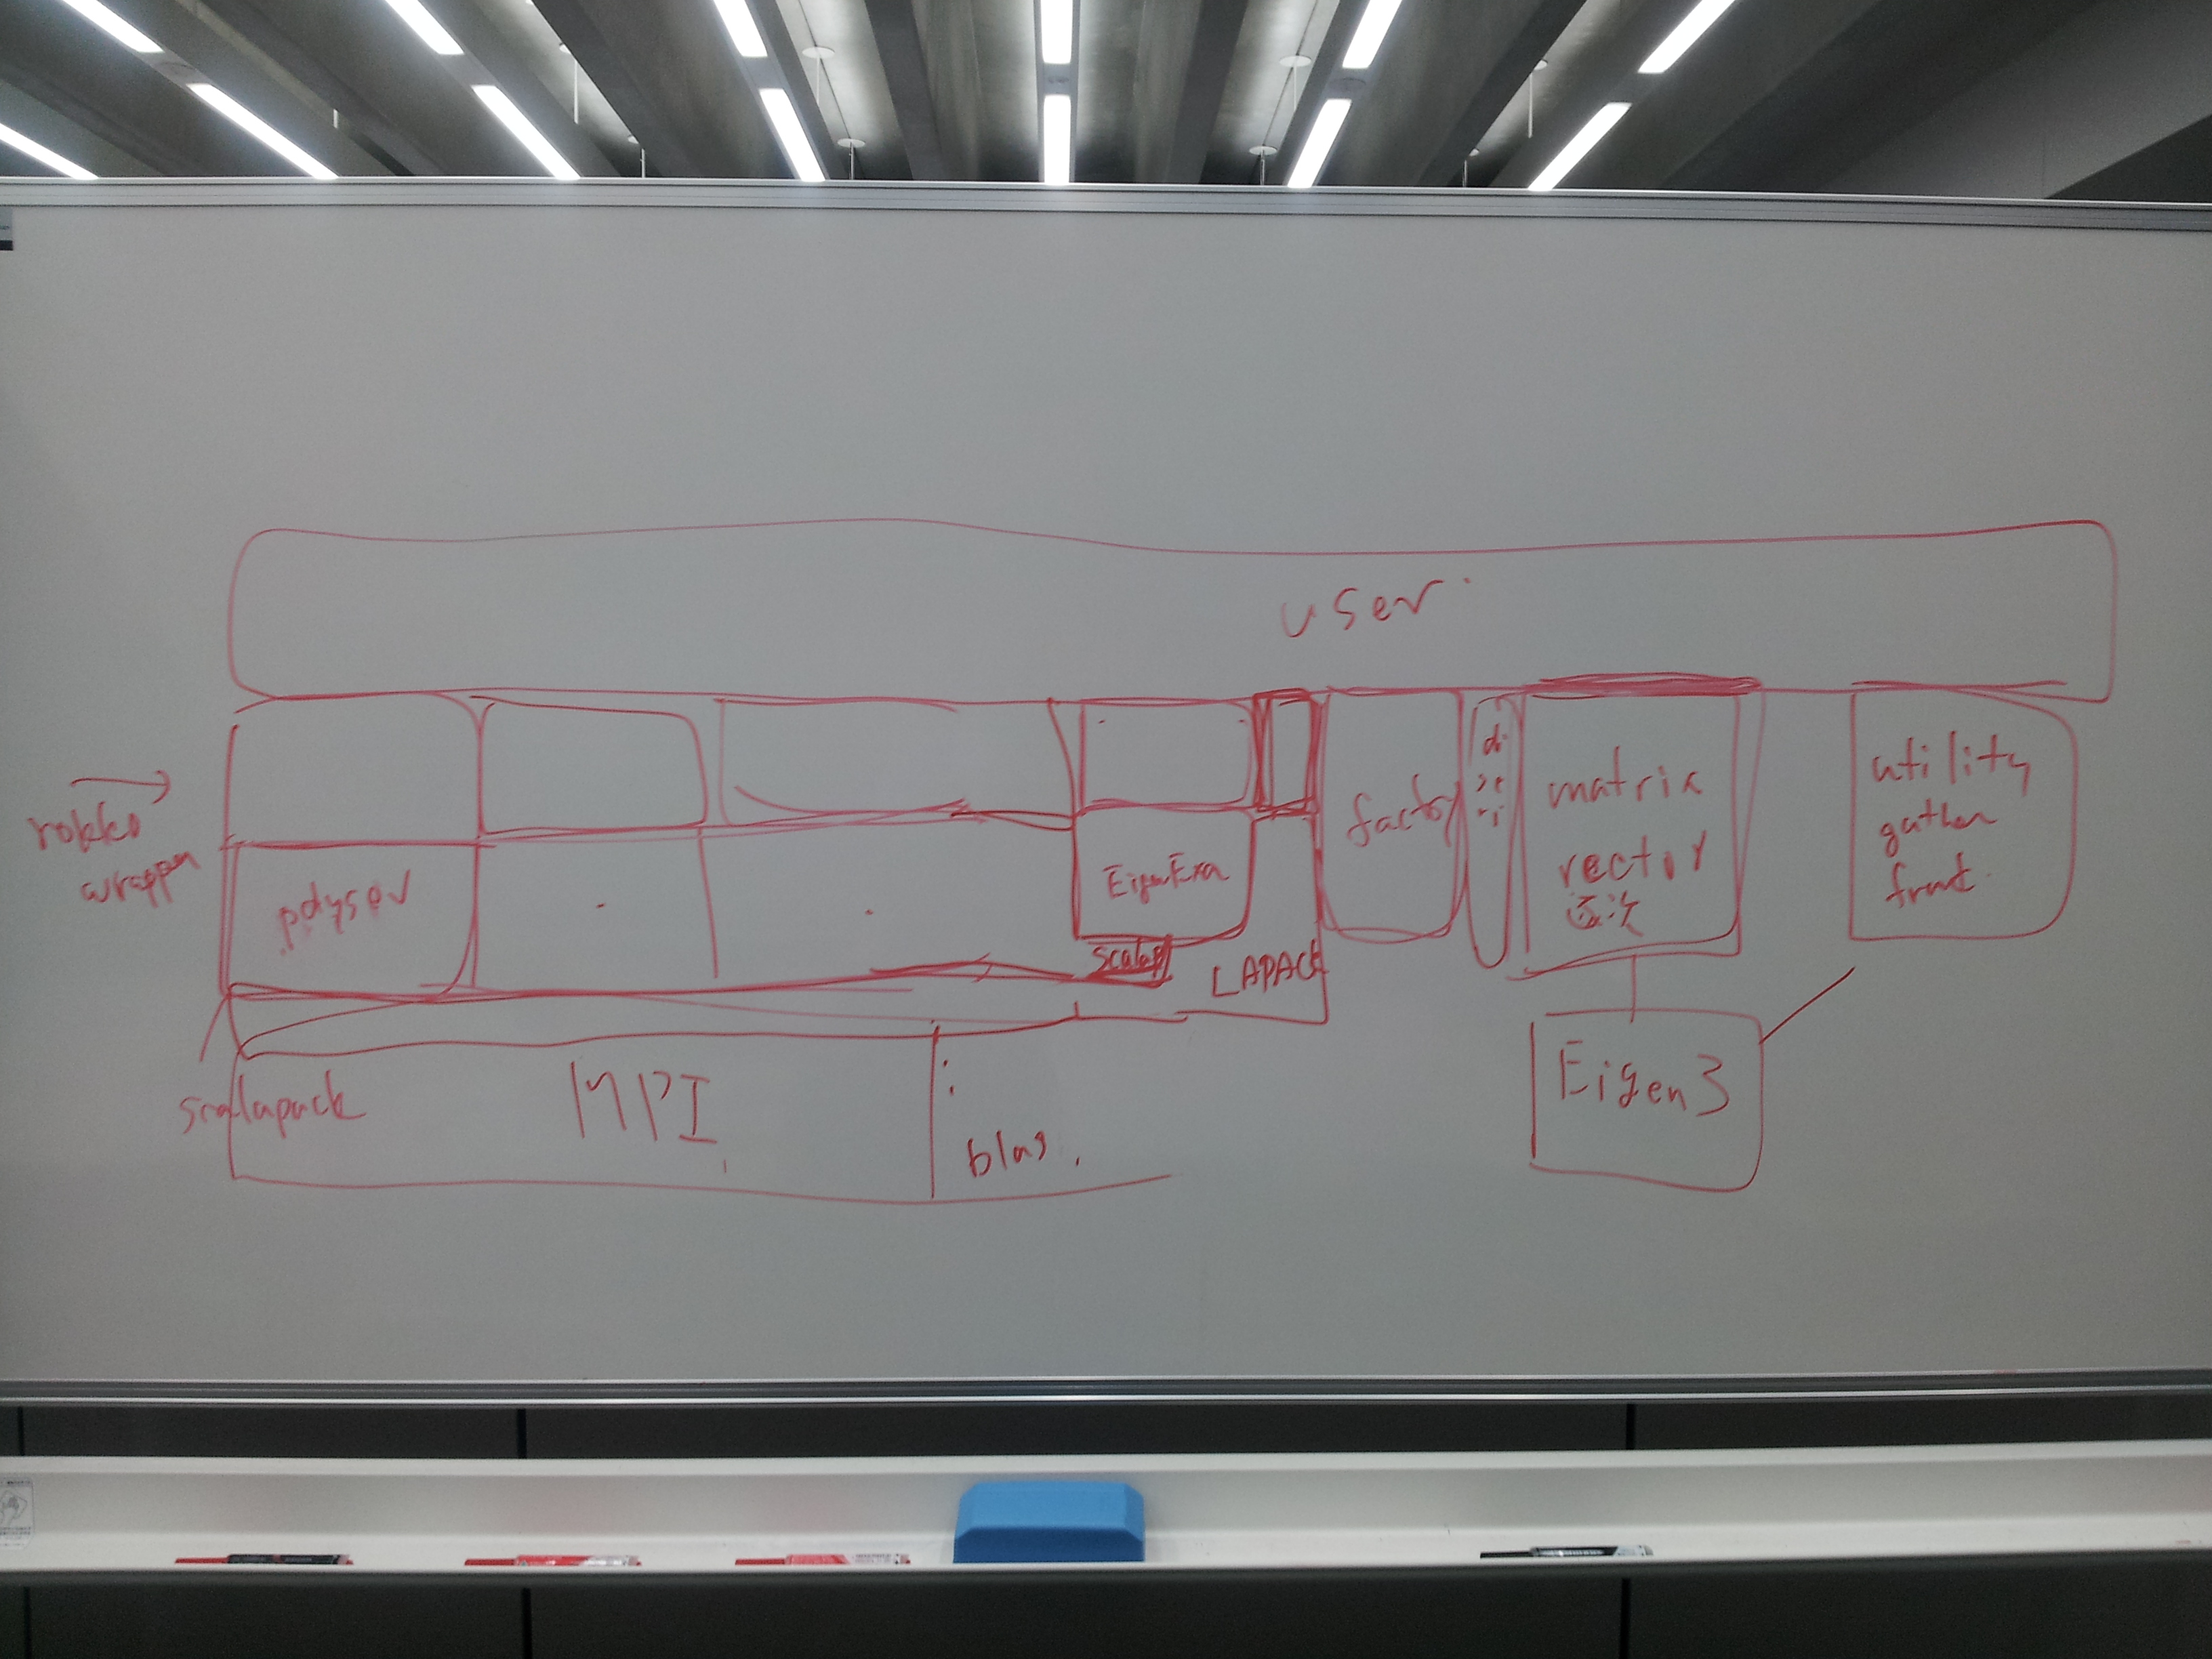
\includegraphics[height=0.8\textheight]{figure/rokko-software-stack.jpg}
  \end{center}
\end{frame}

\section{Rokkoのインストール}

\begin{frame}
  \frametitle{インストール作業に必須のツールとライブラリ}
  \begin{itemize}
    \setlength{\itemsep}{1em}
  \item CMake: \url{http://www.cmake.org}
  \item Boost C++ Libraries: \url{http://www.boost.org}
  \item インストールスクリプト: \url{https://github.com/wistaria/MateriAppsInstaller}
  \item 主要なスパコンへのインストール状況 \\
    \url{https://github.com/wistaria/MateriAppsInstaller/wiki}
  \end{itemize}
\end{frame}

\begin{frame}
  \frametitle{ビルドシステム: CMake}
  \begin{itemize}
    \setlength{\itemsep}{1em}
  \item Makefileを生成するためのユーティリティー (configureスクリプトに対応)
    \begin{itemize}
    \item Windows の Visual C++ 用ソリューションファイル, Mac OS X の Xcode 用プロジェクトファイルの生成も可能
    \end{itemize}
  \item 設定は CMakeLists.txt に記述する
  \item テスト(CTest)やバイナリ配布(CPack)の機能もある
  \item ファイルの依存関係の自動検出
  \item ソースディレクトリとビルドディレクトリの分離(バージョン管理がしやすくなる)
  \end{itemize}
\end{frame}

\begin{frame}
  \frametitle{サードパーティーの固有値ソルバ/線形計算ライブラリのインストール}
  \begin{itemize}
    \setlength{\itemsep}{1em}
  \item Eigen3 (ベクトル, 行列クラスを内部で利用), LAPACKE (LAPACKのCインターフェース)は, Rokkoに同梱されている
  \item インストールスクリプト: \href{https://github.com/t-sakashita/rokko/tree/master/3rd-party/install}{3rd-party/install}
    \begin{itemize}
      \item ライブラリ: Anasazi, EigenExa, Elemental, ELPA, PETSc, ScaLAPACK, SLEPc
      \item 対応アーキテクチャ: 京/FX10, x86スパコン・クラスタ(Intelコンパイラ/GCC), Mac OS X (GCC), 他
    \end{itemize}
  \item 主要なスパコンにインストール済み: \url{https://github.com/t-sakashita/rokko/wiki}
  \end{itemize}
\end{frame}

\begin{frame}[c,fragile]
  \frametitle{Rokkoのインストール}
  \begin{itemize}
    %\setlength{\itemsep}{1em}
  \item 下準備 (phi.aics.riken.jpの場合)
\begin{lstlisting}[style=shstyle]
source /home/materiapps/env.sh
source /home/materiapps/rokko/rokkoenv.sh
\end{lstlisting}
  \item ソースコードのダウンロード・展開
\begin{lstlisting}[style=shstyle]
cd $HOME
wget http://github.com/t-sakashita/rokko/archive/0.3.tar.gz -O rokko-0.3.tar.gz
tar zxvf rokko-0.3.tar.gz
\end{lstlisting}
  \item CMakeの実行
\begin{lstlisting}[style=shstyle]
mkdir rokko-build
cd rokko-build
cmake $HOME/rokko-0.3 -DCMAKE_CXX_COMPILER=icpc -DCMAKE_C_COMPILER=icc \
  -DCMAKE_Fortran_COMPILER=ifort -DCMAKE_INSTALL_PREFIX=$HOME/rokko_install
\end{lstlisting}
  \end{itemize}
\end{frame}

\begin{frame}[c,fragile]
  \frametitle{Rokkoのインストール(続き)}
  \begin{itemize}
  \item 上記のコピー&ペーストがうまく行かなかった方は、スクリプトで実行
\begin{lstlisting}[style=shstyle]
cp /home/hands-on/rokko_20150730/cmake-rokko.sh  .
sh cmake-rokko.sh
\end{lstlisting}
  \item Make, テスト
\begin{lstlisting}[style=shstyle]
make -j 4
make test
make install
\end{lstlisting}
  \end{itemize}
\end{frame}

\begin{frame}[c,fragile]
  \frametitle{インストールの成否の確認}
Rokkoで使用できる固有値ルーチン一覧の表示 \RokkoFilename{tool/rokko_solvers.cpp}
\begin{lstlisting}[style=shstyle]
cd $HOME/rokko_install/tool
./rokko_solvers
\end{lstlisting}

出力結果
\begin{lstlisting}[style=shstyle]
[serial dense solvers]
  eigen3
  lapack
[parallel dense solvers]
  eigen_exa
  elemental
  elpa
  scalapack
[parallel sparse solvers]
  anasazi
  slepc
\end{lstlisting}

\end{frame}

\begin{frame}[c,fragile]
  \frametitle{Rokkoのディレクトリ構造}

\dirtree{%
 .1 \RokkoFilename{}.
 .2
 \RokkoFilename{rokko}
 $\cdots$ Rokko本体(ヘッダファイル・ソースファイル).
 .2
 \RokkoFilename{example}
 $\cdots$ サンプルプログラム.
 .3 \RokkoFilename{cxx}.
 .4
 \href{https://github.com/t-sakashita/rokko/tree/develop/example/cxx/dense}{dense}
 $\cdots$ 密行列用(逐次版、MPI版).
 .4 \href{https://github.com/t-sakashita/rokko/tree/develop/example/cxx/sparse}{sparse} $\cdots$ 疎行列用(MPI版).
 .3 \href{https://github.com/t-sakashita/rokko/tree/develop/example/c}{c}.
 .4 \href{https://github.com/t-sakashita/rokko/tree/develop/example/c/dense}{dense} $\cdots$ 密行列用(逐次版、MPI版).
 .4
 \href{https://github.com/t-sakashita/rokko/tree/develop/example/c/sparse}{sparse}
 $\cdots$ 疎行列用(MPI版).
 .3 \href{https://github.com/t-sakashita/rokko/tree/develop/example/fortran}{fortran}.
 .4 \href{https://github.com/t-sakashita/rokko/tree/develop/example/fortran/dense}{dense} $\cdots$ 密行列用(逐次版、MPI版).
 .4 \href{https://github.com/t-sakashita/rokko/tree/develop/example/fortran/sparse}{sparse} $\cdots$ 疎行列用(MPI版).
% .2
% \href{https://github.com/t-sakashita/rokko/tree/develop/test}{test}
% $\cdots$ ctest用(インストール成否の確認).
% .2 3rd-party $\cdots$ 固有値ソルバ.
 .2 \href{https://github.com/t-sakashita/rokko/tree/develop/tutorial}{tutorial} $\cdots$ チュートリアル.
 .3
 \href{https://github.com/t-sakashita/rokko/tree/develop/tutorial/titpack}{titpack}
 $\cdots$ 厳密対角化パッケージの書き換え.
}

\end{frame}

\section{密行列向け逐次ソルバ}

\subsection*{Rokkoインターフェースの仕様}

\begin{frame}[c,fragile]
  \frametitle{rokko::localized\_matrix クラステンプレート}
  \begin{itemize}
  \item \RokkoFilename{rokko/localized_matrix.hpp}
\begin{lstlisting}
namespace rokko {
template<typename T, typename MATRIX_MAJOR = rokko::matrix_col_major>
class localized_matrix {
public:
  typedef T value_type;
  MATRIX_MAJOR major_type;
  typedef MATRIX_MAJOR major_type;
  localized_matrix();
  localized_matrix(int rows, int cols);
  template <typename U>
  localized_matrix(U const& other);
  template <typename U>
  matrix_type& operator=(U const& other);
  double operator[](int i, int j) const;
  double& operator[](int i, int j);
  int get_m_global() const;
  int get_n_global() const;
  int get_m_local() const;
  int get_n_local() const;
  bool is_gindex_myrow(const int& global_i) const;
};
}
\end{lstlisting}
  \end{itemize}
\end{frame}

\begin{frame}[c,fragile]
  \frametitle{rokko::localized\_vector と rokko::localized\_matrix の利用例}
  \begin{itemize}
  \item \RokkoFilename{test/localized\_matrix.cpp}
\begin{lstlisting}
int dim = 3;
rokko::localized_matrix<double> M(dim,dim);
M << 1,2,3,4,5,6,7,8,9;
double a = 5.0;
rokko::localized_vecto<double>r u(dim);
u << 1,2,3;
rokko::localized_vector<double> v(dim);
v << 4,5,6;
rokko::localized_vector<double> w = a*u+M*v;
\end{lstlisting}
  \end{itemize}
\end{frame}

\begin{frame}[c,fragile]
  \frametitle{rokko::serial_dense_solverクラス}
  \begin{itemize}
    %\setlength{\itemsep}{1em}
  \item ソルバの初期化
\begin{lstlisting}
rokko::serial_dense_solver solver(name);
solver.initialize(argc, argv);
\end{lstlisting}
  \item ソルバの終了
\begin{lstlisting}
solver.finalize();
\end{lstlisting}
  \item 対角化 (行列は破壊される)
\begin{lstlisting}
rokko::localized_matrix<double, matrix_col_major> mat(dim, dim);
...
rokko::localized_vector<double> evals(dim);
rokko::localized_matrix<double, matrix_col_major> evecs(dim, dim);
solver.diagonalize(mat, eigval, eigvec, params);
\end{lstlisting}
%  \item 登録されているソルバの一覧
%\begin{lstlisting}
%std::vector<std::string> names = rokko::serial_dense_solver::solvers();
%\end{lstlisting}
  \end{itemize}
\end{frame}

\subsection*{サンプルの実行}

\begin{frame}[c,fragile]
  \frametitle{対角化のサンプル}
  \begin{itemize}
    %\setlength{\itemsep}{1em}
%  \item 逐次密行列ソルバーの一覧 \href{https://github.com/t-sakashita/rokko/blob/master/test/serial_dense_solvers.cpp}{test/serial\_dense\_solvers.cpp}
%\begin{lstlisting}[style=shstyle]
%./test/serial_dense_solvers
%\end{lstlisting}
  \item LAPACK dsyev を直接使う \RokkoFilename{example/cxx/dense/dsyev.c}
\begin{lstlisting}[style=shstyle]
./example/cxx/dense/dsyev
\end{lstlisting}
逐次密行列ソルバを使う
  \item C++版 \RokkoFilename{example/cxx/dense/frank.cpp}
\begin{lstlisting}[style=shstyle]
./example/cxx/dense/frank lapack 5
\end{lstlisting}
  \item C版 \RokkoFilename{example/c/dense/frank.c}
\begin{lstlisting}[style=shstyle]
./example/c/dense/frank lapack 5
\end{lstlisting}
  \item Fortran版 \RokkoFilename{example/fortran/dense/frank.f90}
\begin{lstlisting}[style=shstyle]
./example/fortran/dense/frank lapack 5
\end{lstlisting}
  \end{itemize}
\end{frame}

\begin{frame}[c,fragile]
   \frametitle{固有値ソルバへのパラメータの渡し方}
   \begin{itemize}
   \item パラメータクラス\RokkoFilename{rokko/parameters.hpp}を利用
     \begin{itemize}
     \item \RokkoFilename{example/cxx/dense/frank.cpp}の例:
\begin{lstlisting}
   rokko::parameters params;
   params.set("routine", "tri");
   params.set("upper_value", 1.2);
   params.set("lower_value", 0.1);
   params.set("uplow", "lower");
   params.set("verbose", true);
\end{lstlisting}
\end{itemize}
   \end{itemize}
\end{frame}

\begin{frame}[c,fragile]
  \frametitle{密行列逐次ソルバに渡すパラメータ}
Eigen3\\
\scalebox{0.55}{
\begin{tabular}[c]{|c|c|c|c|c|c|c|}
\hline
Rokkoルーチン名 & 元のルーチン名 & 解法 & 入力パラメータ(オプション) & 出力パラメータ & 備考\\
\whline
eigen3:qr & SelfAdjointEigensolver & QR法 & なし & なし & デフォルト\\
\hline
\end{tabular}
}
\end{frame}

\begin{frame}[c,fragile]
  \frametitle{密行列逐次ソルバに渡すパラメータ}
LAPACK\\
\scalebox{0.55}{
\begin{tabular}[c]{|c|c|c|c|c|c|c|}
\hline
Rokkoルーチン名 & 元のルーチン名 & 解法 & \parbox{2.5cm}{入力パラメータ\\(オプション)} & 出力パラメータ & 備考\\
\whline
\parbox{2cm}{lapack:dsyev\\lapack:qr} & dsyev & QR法 & uplow & なし & 引数なしのデフォルト\\
\hline
lapack:dsyevx & dsyevx & \parbox[c]{1.5cm}{2分法\\QR法} & \parbox{3.5cm}{upperとlowerの組,\\abstol, uplow} & m, ifail & \parbox{5cm}{$abstol>0$のとき、2分法,\\$abstol<0$のとき、QR法}\\
\hline
lapack:bisection & dsyevx & 2分法 & \parbox{3.5cm}{upperとlowerの組,\\abstol, uplow} & m, fail & dsyevxを$abstol>0$で使用\\
\hline
\parbox{2cm}{lapack:dsyevr\\lapack:mr3} & dsyevr & MR3法 & \parbox{3.5cm}{upperとlowerの組,\\abstol, uplow} & m, isuppz & 固有値範囲指定ありのデフォルト\\
\hline
\parbox{2cm}{lapack:dsyevd\\lapack:dc} & dsyevd & 分割統治法 & uplow & なし & \\
\hline
\end{tabular}
}

LAPACK向け入力パラメータ
\scalebox{0.55}{
\begin{tabular}[c]{|c|c|c|c|c|c|c|}
\hline
\parbox{2.5cm}{Rokkoの\\パラメータ名} & \parbox{2.5cm}{ScaLAPACKの\\パラメータ名} & 型 & 意味 & 値 & 備考\\
\whline
matrix_part & uplow & std::string & \parbox{4cm}{ソルバに読まれる部分\\(上三角/下三角)} & \parbox{1.5cm}{upper(U),\\lower(L)} & \parbox{5cm}{最初の一文字で判断。\\大文字、小文字のどちらも可。\\デフォルトは、'U' } \\
\hline
abstol & abstol & double & 固有値の収束判定に用いる & & \\
\hline
upper_index & iu & int & 求めたい固有値の番号の上限 & & 番号は昇順につけられる\\
\hline
upper_value & vu & double & 求めたい固有値の範囲の上限 & & \\
\hline
lower_index & il & int & 求めたい固有値の番号の下限 & & 番号は昇順につけられる\\
\hline
lower_value & vl & double & 求めたい固有値の範囲の下限 & & \\
\hline
verbose     & なし & bool & \parbox{5cm}{Rokkoで用意したフラグ。\\ソルバに設定した入力パラメータ、エラーの詳細を表示。} & & デフォルトはfalse\\
\hline
\end{tabular}
}
\end{frame}

\section{密行列向けMPI並列ソルバ}

\subsection*{基本概念}

\begin{frame}
  \frametitle{2次元プロセスグリッド}
  \begin{itemize}
    %\setlength{\itemsep}{1em}
  \item MPIプロセスの2次元割付けを指定
  \item Row-majorとcolumn-majorの二種類
  \item 4プロセスの例 (左:row-major, 右:column-major)
  \begin{center}
    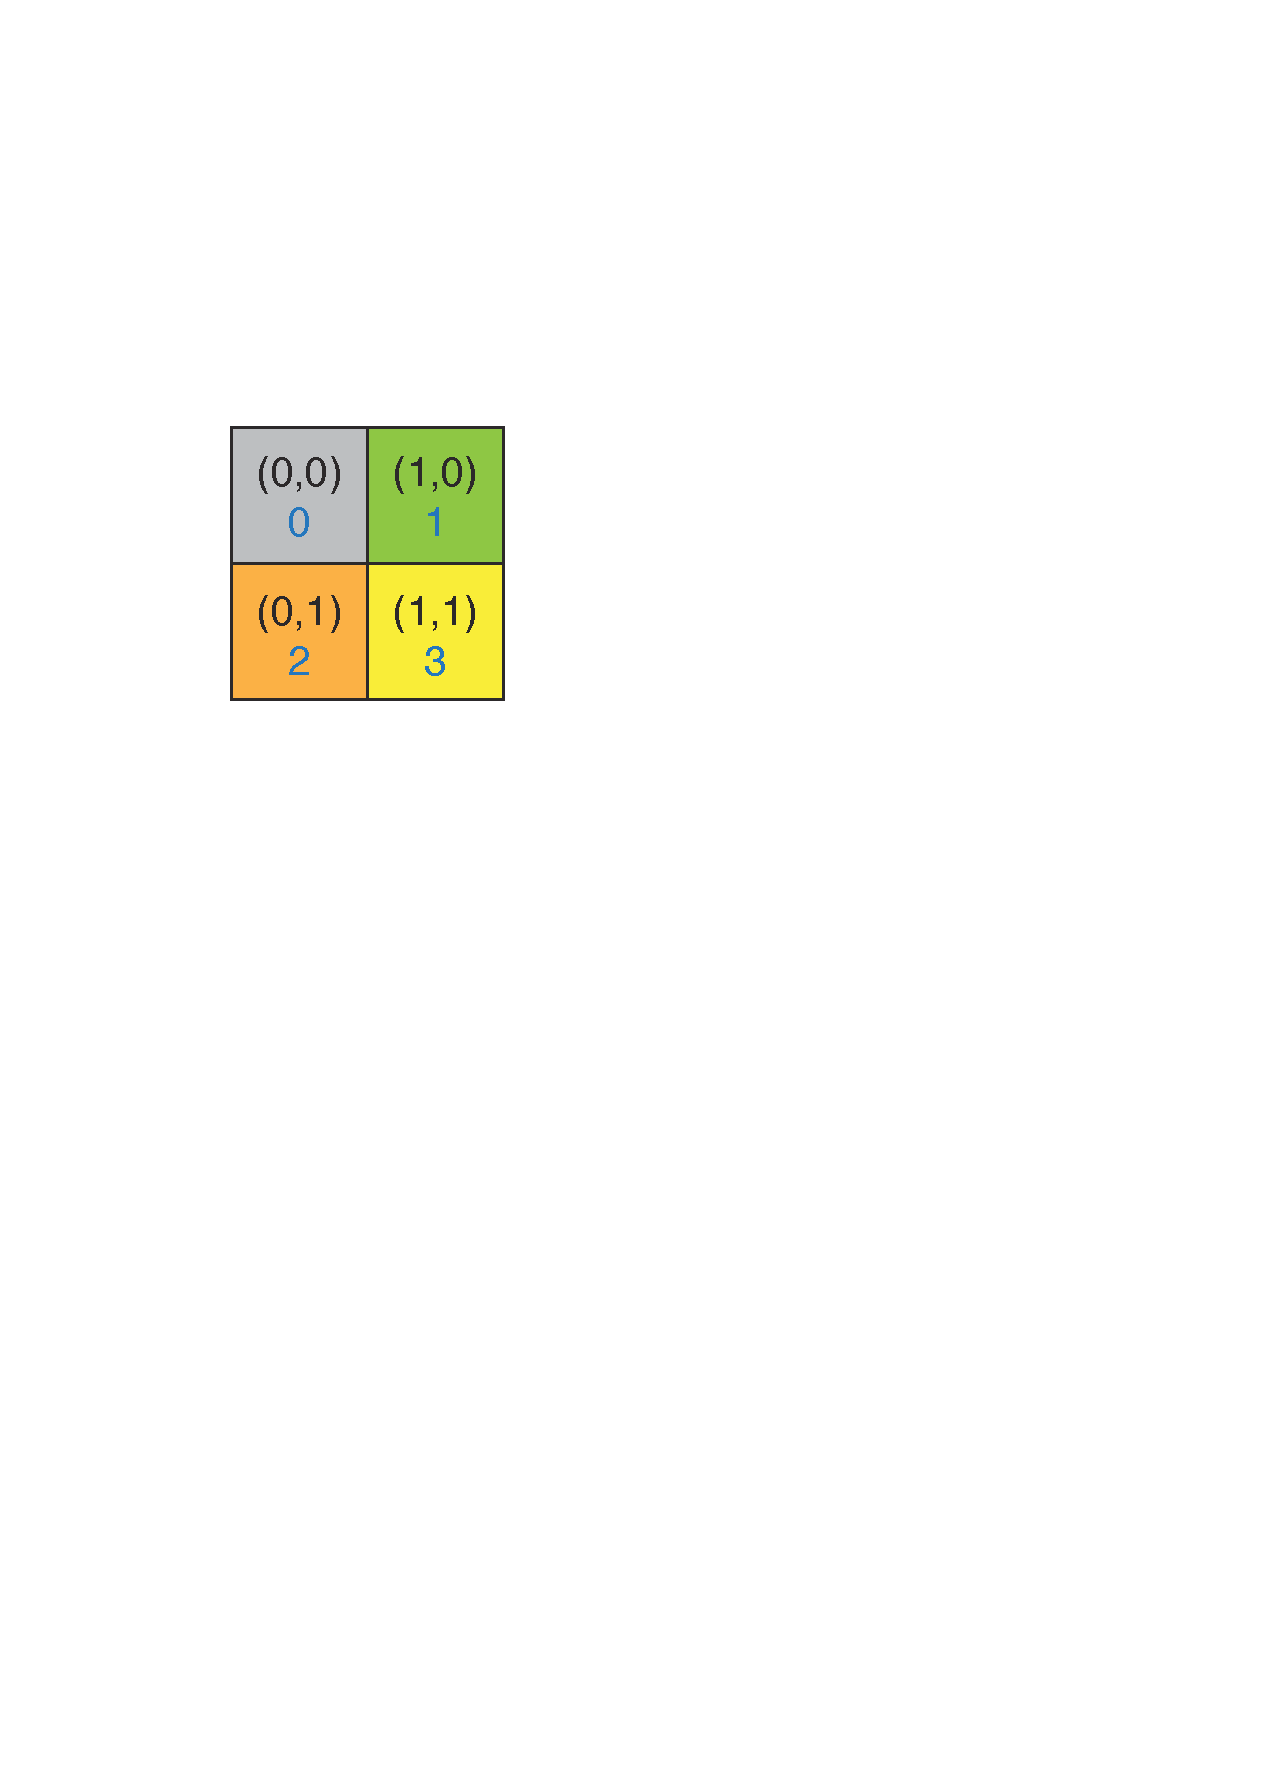
\includegraphics[height=0.25\textheight]{figure/grid-row-major.pdf} \ \ \ \
    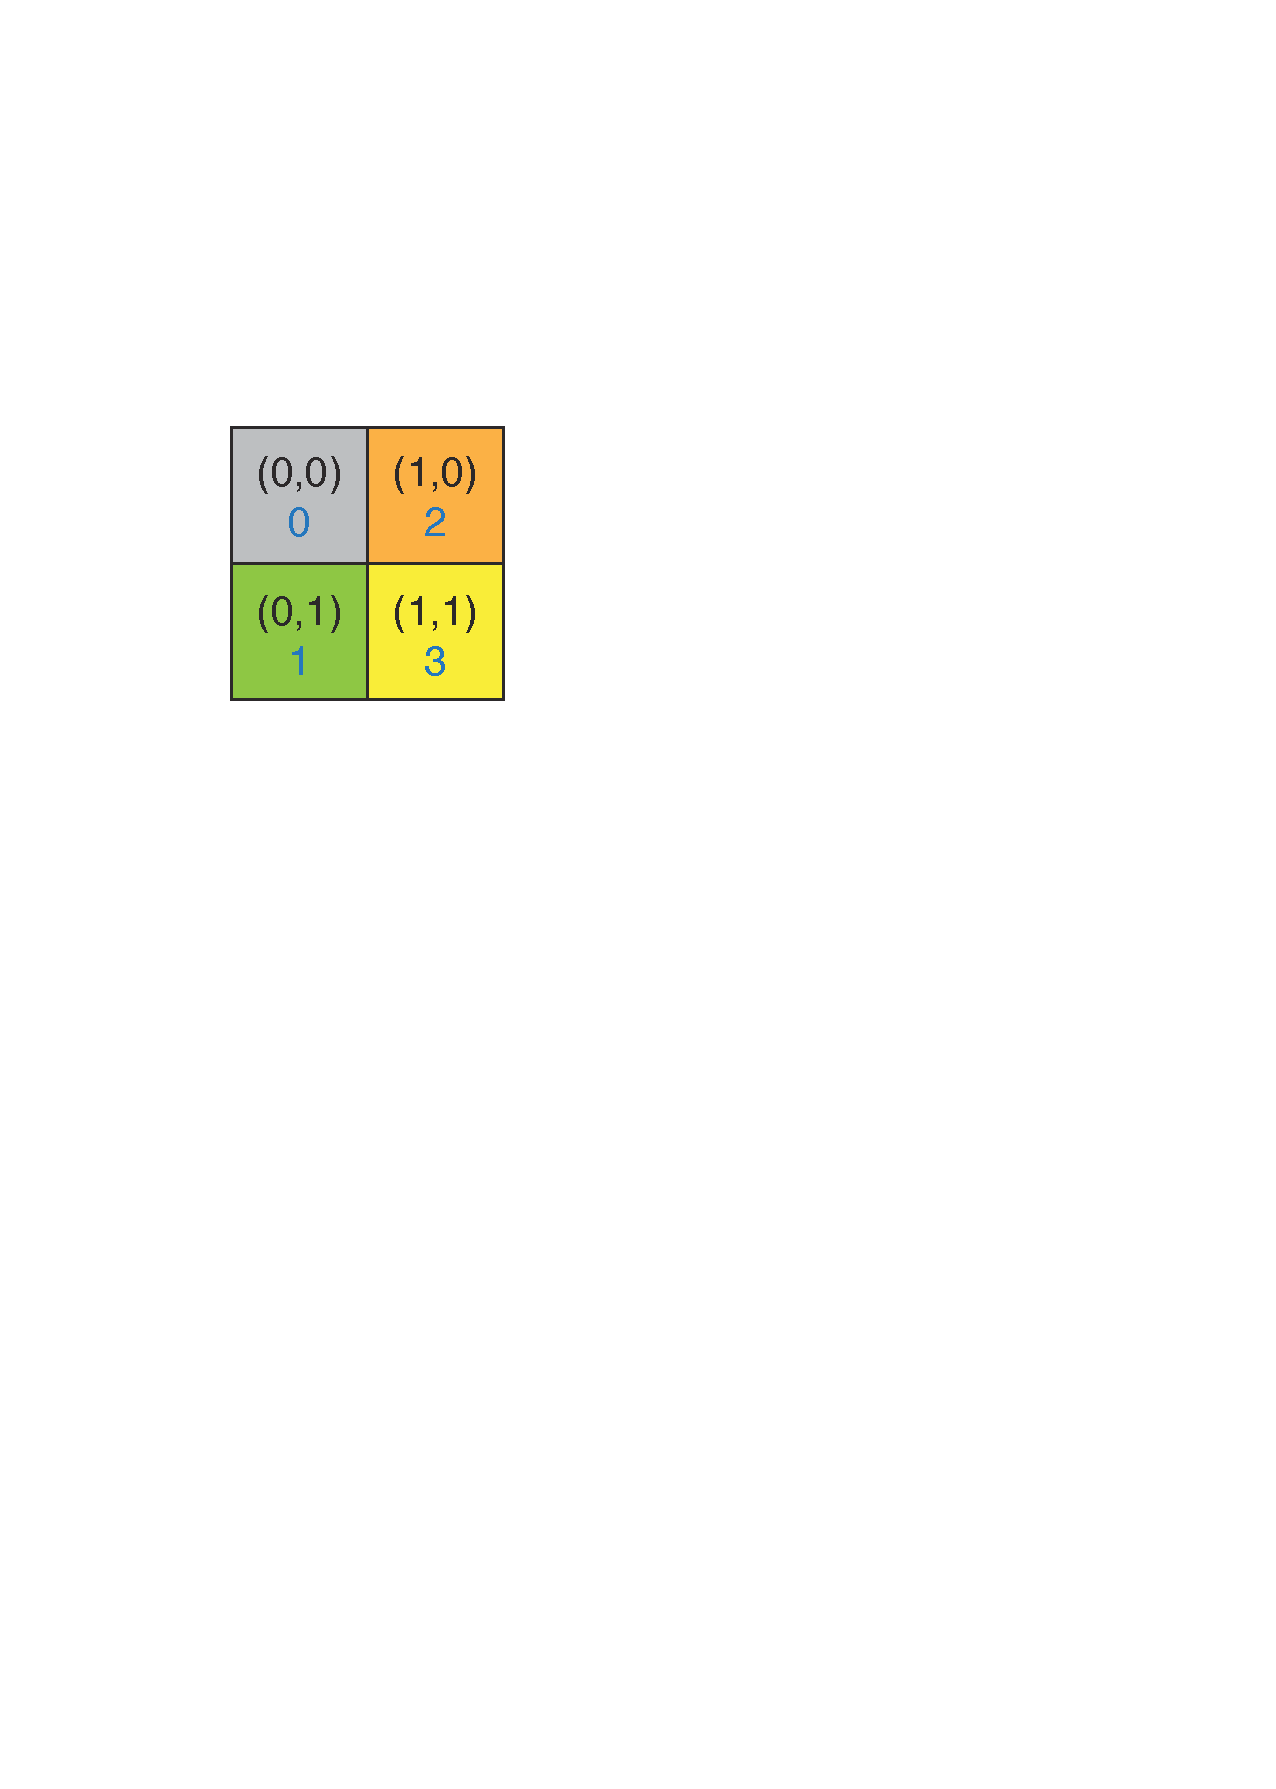
\includegraphics[height=0.25\textheight]{figure/grid-column-major.pdf}
  \end{center}
  \item 全てのソルバは両方の種類をサポート
  \end{itemize}
\end{frame}

\begin{frame}
  \frametitle{2次元ブロック・サイクリック行列(distributed\_matrix)}
  \begin{itemize}
    %\setlength{\itemsep}{1em}
  \item ほとんどの並列固有値ソルバにおいて, 密行列は「2次元ブロック・サイクリック形式」でデータ分割される
  \item 4プロセスでの例 (左 ローカルビュー, 右 グローバルビュー)
  \begin{center}
    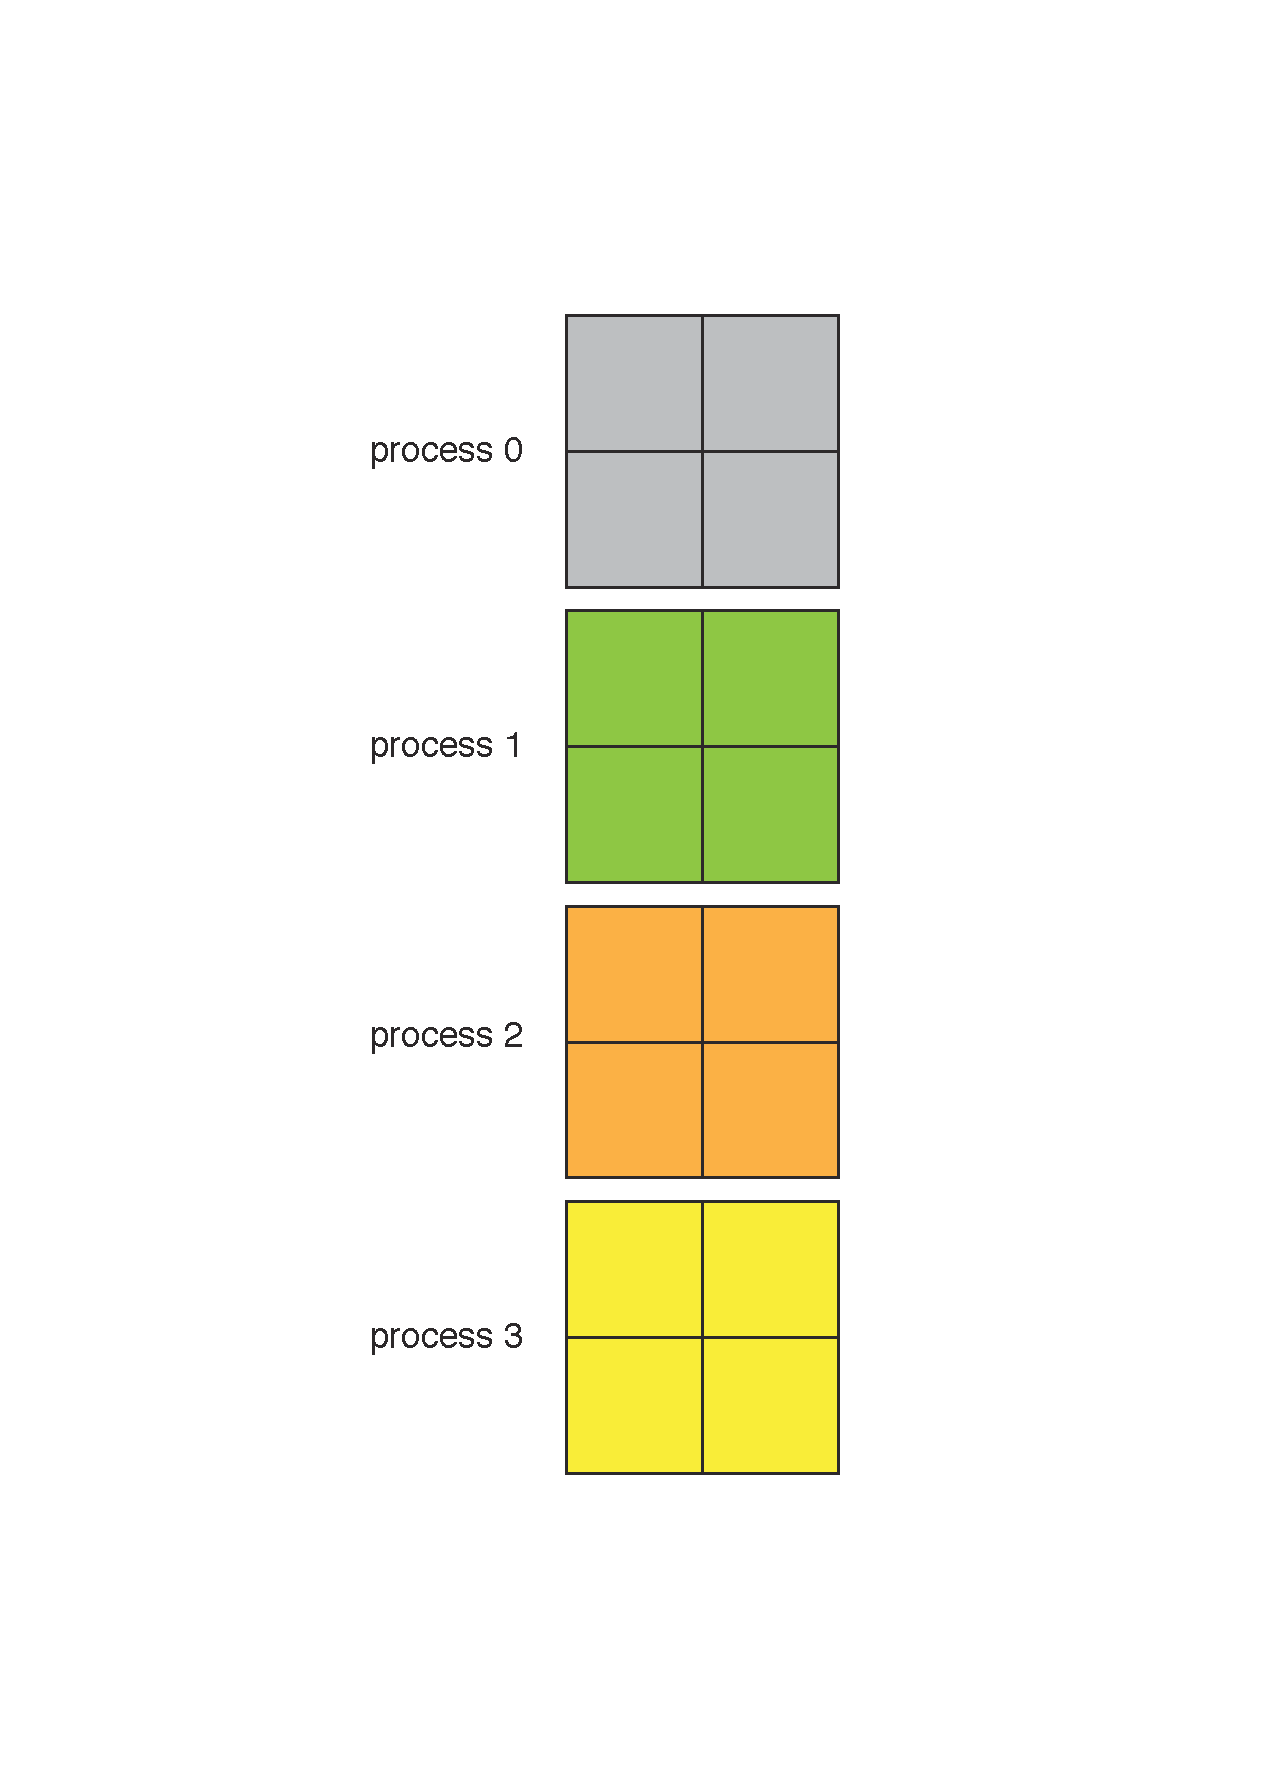
\includegraphics[height=0.45\textheight]{figure/local-view.pdf} \ \ \ \ \ \ \ \
    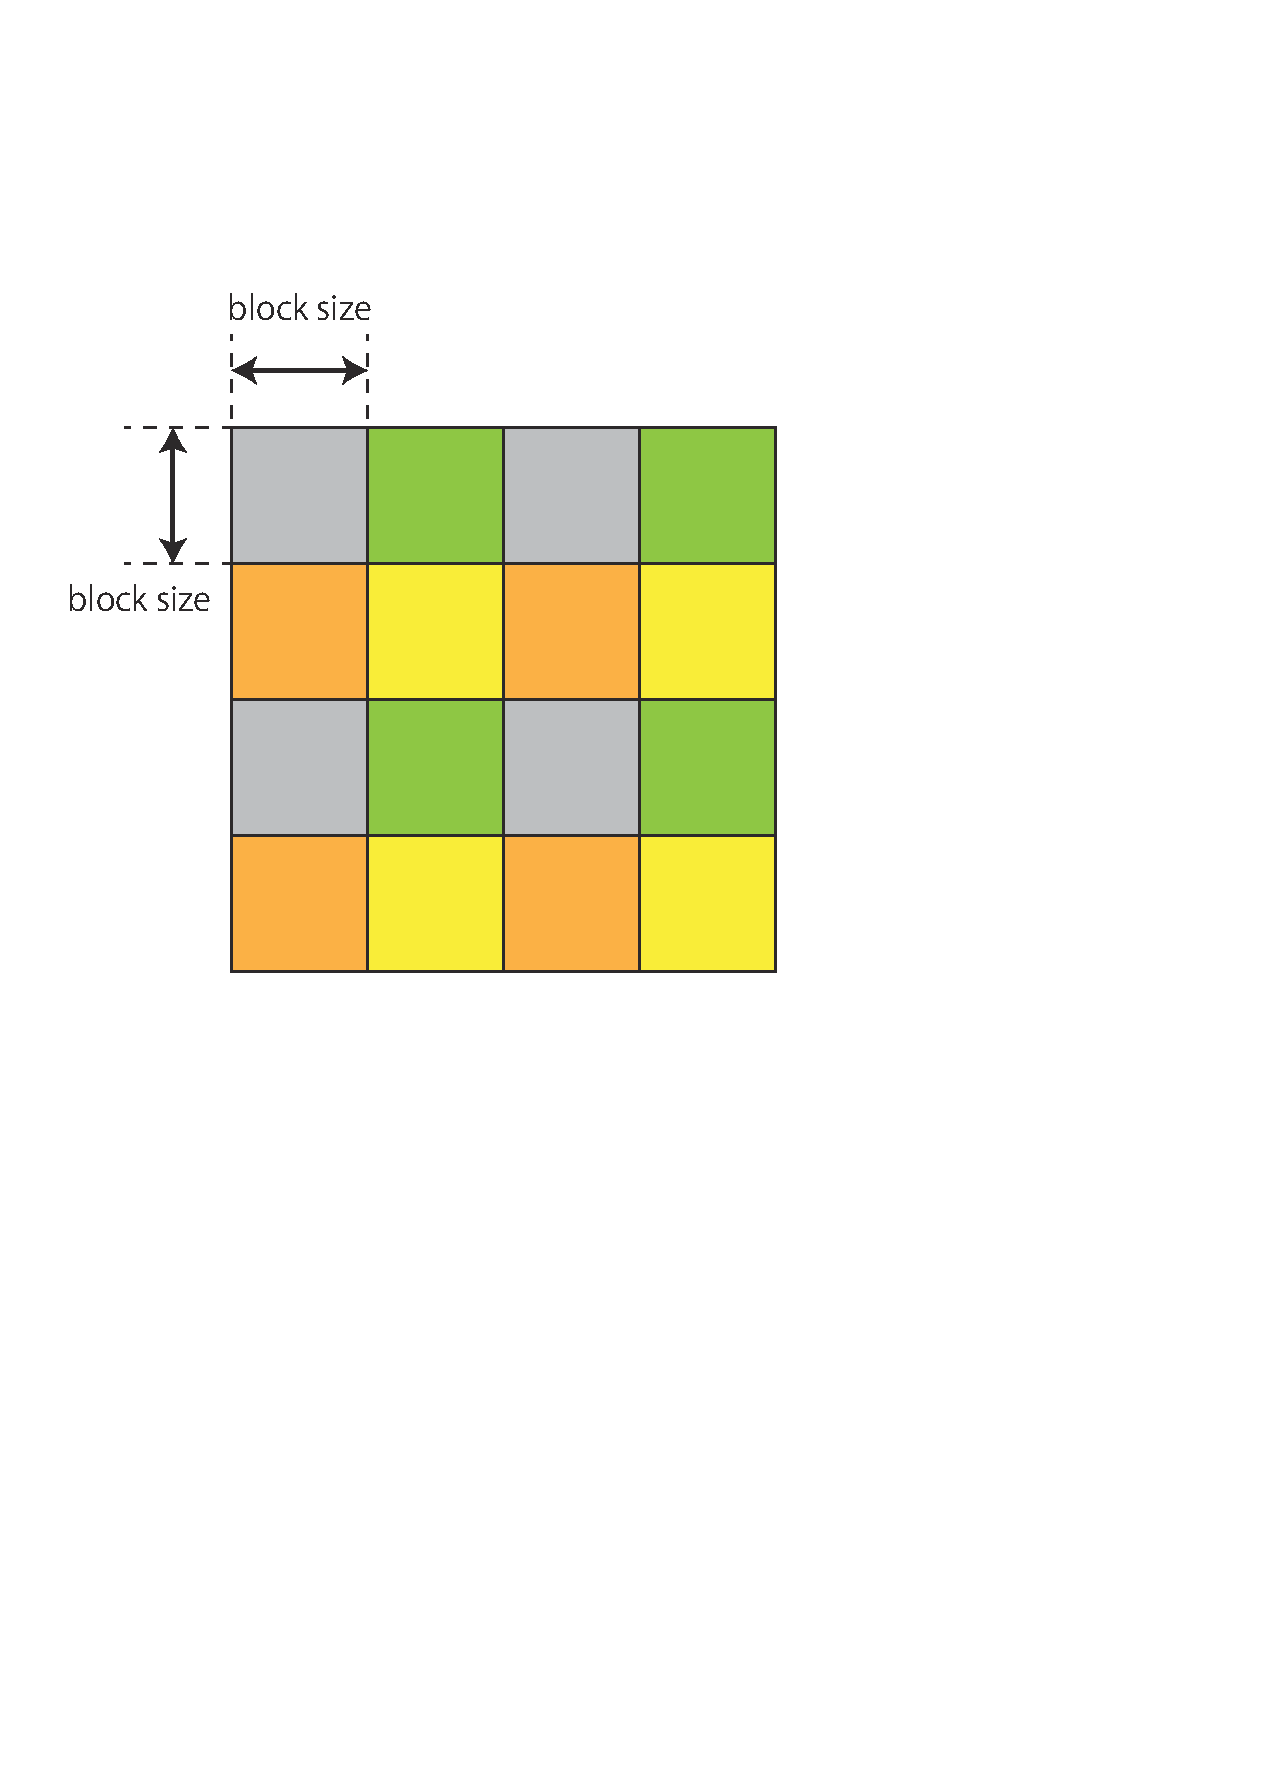
\includegraphics[height=0.35\textheight]{figure/global-view.pdf}
  \end{center}
  \item ScaLAPACKとELPAは任意のブロックサイズをサポート
  \item EigenExaとElementalは$1 \times 1$のみをサポート
  \end{itemize}
\end{frame}

\subsection*{Rokkoインターフェースの仕様}

\begin{frame}[c,fragile]
  \frametitle{rokko::grid クラス}
  \begin{itemize}
  \item \RokkoFilename{rokko/grid.hpp}
\begin{lstlisting}
namespace rokko {
extern struct grid_row_major_t {} grid_row_major;
extern struct grid_col_major_t {} grid_col_major;
class grid {
public:
  explicit grid(MPI_Comm comm_in = MPI_COMM_WORLD);
  template <typename GRID_MAJOR>
  grid(MPI_Comm comm_in, GRID_MAJOR const& grid_major);
  MPI_Comm get_comm() const { return comm; }
  int get_nprocs() const;
  int get_nprow() const;
  int get_npcol() const;
  int get_myrank() const;
  int get_myrow() const;
  int get_mycol() const;
  bool is_row_major() const;
  bool is_col_major() const;
  int calculate_grid_row(int proc_rank) const;
  int calculate_grid_col(int proc_rank) const;
};
}
\end{lstlisting}
  \end{itemize}
\end{frame}


\begin{frame}[c,fragile]
  \frametitle{rokko::distributed_matrix クラステンプレート}
  \begin{itemize}
  \item \RokkoFilename{rokko/distributed_matrix.hpp}
\begin{lstlisting}
namespace rokko {
template<typename T, typename MATRIX_MAJOR = rokko::matrix_col_major>
class distributed_matrix {
public:
  template<typename SOLVER>
  distributed_matrix(mapping_bc<MATRIX_MAJOR> const& map_in);
  template<typename SOLVER>
  ...
  bool is_gindex_myrow(int global_i) const; // プロセスグリッドのうち、自プロセスの行方向の番号を返す
  bool is_gindex_mycol(int global_j) const; // プロセスグリッドのうち、自プロセスの列方向の番号を返す
  bool is_gindex(int global_i, int global_j) const; // 自プロセスが(global_i, global_j)を持っているか?
  void set_local(int local_i, int local_j, double value);  // 自プロセスのlocal storageの(local_i, local_j)に値valueを格納
  double get_local(int local_i, int local_j) const;  // 自プロセスのlocal storageの(local_i, local_j)の値を返す
  void update_local(int local_i, int local_j, double value); // 自プロセスのlocal storageの(local_i, local_j)に値valueを足し込む
  void set_global(int global_i, int global_j, double value); // 自プロセスが(global_i, global_j)を受け持っていたら、値valueを格納
  double get_global(int global_i, int global_j) const; // 自プロセスが(global_i, global_j)を受け持っていたら、その値を返す
};
}
\end{lstlisting}
  \end{itemize}
\end{frame}

\begin{frame}[c,fragile]
  \frametitle{distributed\_matrixの操作}
  \begin{itemize}
    %\setlength{\itemsep}{1em}
  \item 行列の掛け算 $C = \alpha A B + \beta C$
\begin{lstlisting}
  ...
  rokko::mapping_bc<matrix_major> map(dim, g, solver);  // 正方行列と与えられたgridとsolverに適切なブロックサイズを返す。
  rokko::distributed_matrix<double, rokko::matrix_col_major> matA(map);
  rokko::distributed_matrix<double, rokko::matrix_col_major> matB(map);
  rokko::distributed_matrix<double, rokko::matrix_col_major> matC(map);
  ...
  rokko::product(alpha, matA, transA, matB, transB, beta, matC);
\end{lstlisting}
  \item distributed\_matrixの scatter と gather
\begin{lstlisting}
  rokko::localized_matrix<double, LOC_MAT_MAJOR> lmat(dim, dim);
  rokko::distributed_matrix<double, DIST_MAT_MAJOR> mat(map);
  rokko::scatter(lmat, mat, root);
  rokko::gather(mat, lmat, root);
\end{lstlisting}
  \end{itemize}
\end{frame}

\begin{frame}[c,fragile]
  \frametitle{distributed_matrixの生成}
  \begin{itemize}
    %\setlength{\itemsep}{1em}
  \item 要素毎に代入 (globalな添字)
\begin{lstlisting}
for(int global_i=0; global_i < mat.get_m_global(); ++global_i) {
  for(int global_j=0; global_j < mat.get_n_global(); ++global_j) {
    mat.set_global(global_i, global_j, f(global_i, global_j));
  }
}
\end{lstlisting}
  \item 要素毎に代入 (localな添字)
\begin{lstlisting}
for(int local_i = 0; local_i < mat.get_m_local(); ++local_i) {
  for(int local_j = 0; local_j < mat.get_n_local(); ++local_j) {
    int global_i = mat.translate_l2g_row(local_i);
    int global_j = mat.translate_l2g_col(local_j);
    mat.set_local(local_i, local_j, f(global_i, global_j));
  }
}
\end{lstlisting}
  \item 関数の値で行列を埋める
\begin{lstlisting}
mat.generate(f);
\end{lstlisting}
  \end{itemize}
\end{frame}

\begin{frame}[c,fragile]
  \frametitle{rokko::parallel_dense_solverクラス}
  \begin{itemize}
    %\setlength{\itemsep}{1em}
  \item ソルバの初期化
\begin{lstlisting}
rokko::parallel_dense_solver solver(name);
solver.initialize(argc, argv);
\end{lstlisting}
  \item ソルバの終了
\begin{lstlisting}
solver.finalize();
\end{lstlisting}
  \item 対角化 (行列は破壊される)
\begin{lstlisting}
rokko::mapping_bc<double, matrix_major> map(dim, g, solver);
rokko::distributed_matrix<double, matrix_col_major> mat(map);
...
rokko::localized_vector evals(dim);
rokko::distributed_matrix<double, matrix_col_major> evecs(map);
solver.diagonalize(mat, evals, evecs, params);
\end{lstlisting}
%  \item 登録されているソルバの一覧
%\begin{lstlisting}
%std::vector<std::string> names = rokko::parallel_dense_solver::solvers();
%\end{lstlisting}
  \end{itemize}
\end{frame}

\subsection*{サンプルの実行}

\begin{frame}[c,fragile]
  \frametitle{対角化のサンプル}
  \begin{itemize}
    %\setlength{\itemsep}{1em}
%  \item MPI並列密行列ソルバーの一覧 \href{https://github.com/t-sakashita/rokko/blob/master/test/parallel_dense_solvers.cpp}{test/parallel_dense_solvers.cpp}
%\begin{lstlisting}[style=shstyle]
%./test/parallel_dense_solvers
%\end{lstlisting}
  \item C++ \RokkoFilename{example/cxx/dense/frank_mpi.cpp}
\begin{lstlisting}[style=shstyle]
mpirun -np 4 ./example/cxx/dense/frank_mpi eigen_exa 5
\end{lstlisting}
  \item C版 \RokkoFilename{example/c/dense/frank_mpi.cpp}
\begin{lstlisting}[style=shstyle]
mpirun -np 4 ./example/c/dense/frank_mpi eigen_exa 5
\end{lstlisting}
  \item Fortran版 \RokkoFilename{example/fortran/dense/frank_mpi.cpp}
\begin{lstlisting}[style=shstyle]
mpirun -np 4 ./example/fortran/dense/frank_mpi eigen_exa 5
\end{lstlisting}

\end{itemize}
\end{frame}

\begin{frame}[c,fragile]
  \frametitle{テスト行列:Frank行列(定義)}
\begin{block}{定義}
$[a_{ij}]_{i,j = {0, \dots, n-1}} = [ n - \max(i,j) ]$\\
\end{block}

\begin{block}{Example ($n=5$)}
$[a_{ij}]_{i,j = {0, \dots, 4}} =
\begin{bmatrix}
5 & 4 & 3 & 2 & 1 \\
4 & 4 & 3 & 2 & 1 \\
3 & 3 & 3 & 2 & 1 \\
2 & 2 & 2 & 2 & 1 \\
1 & 1 & 1 & 1 & 1 \\
\end{bmatrix}
$
\end{block}
\end{frame}

\begin{frame}[c,fragile]
  \frametitle{テスト行列:Frank行列(性質)}
\begin{block}{理論固有値}%
$\lambda_k = \dfrac{1}{2 \left( 1 - \cos{\tfrac{2 k + 1}{2 n + 1}\pi} \right)} \quad (k=0,\dots,n-1)$
\end{block}

\begin{block}{}%
Frank matrix has an eigenvalue $1$\\
\quad $\Longleftrightarrow$ $\tfrac{2 k + 1}{2 n + 1} = \tfrac{1}{3}$\\
\quad $\Longleftrightarrow$ $n-1$ is a multiple of 3.
\end{block}
\end{frame}

\setlength{\tabcolsep}{2pt}

\begin{frame}[c,fragile]
  \frametitle{密行列MPI並列ソルバに渡すパラメータ}

ScaLAPACK向けルーチン
\scalebox{0.55}{
\begin{tabular}[c]{|c|c|c|c|c|c|c|}
\hline
 Rokkoルーチン名 & 元のルーチン名 & 解法 & \parbox{2.5cm}{入力パラメータ\\(オプション)} & 出力パラメータ & 備考\\
\whline
\parbox{3cm}{scalapack:pdsyev\\scalapack:qr} & pdsyev & QR法 & uplow & なし & 引数なしのデフォルト\\
\hline
scalapack:pdsyevx & pdsyevx & \parbox[c]{1.5cm}{2分法\\QR法} & \parbox{3.5cm}{upperとlowerの組,\\abstol, uplow}  & m, ifail & \parbox{5cm}{$abstol>0$のとき、2分法,\\$abstol<0$のとき、QR法}\\
\hline
scalapack:bisection & pdsyevx & 2分法 & \parbox{3.5cm}{upperとlowerの組,\\abstol, uplow} & m, ifail & pdsyevxを$abstol>0$として使用\\
\hline
\parbox{3cm}{scalapack:pdsyevr\\scalapack:mr3} & pdsyevr & MR3法 & \parbox{3.5cm}{upperとlowerの組,\\abstol, uplow, orfac} & \parbox[c]{2cm}{m, nz, ifail,\\iclustr, gap} & 固有値範囲指定ありのデフォルト\\
\hline
\parbox{3cm}{scalapack:pdsyevd\\scalapack:dc} & pdsyevd & 分割統治法 & uplow & なし & \\
\hline
\end{tabular}
}

ScaLAPACK向け入力パラメータ
\scalebox{0.55}{
\begin{tabular}[c]{|c|c|c|c|c|c|c|}
\hline
\parbox{2.5cm}{Rokkoの\\パラメータ名} & \parbox{2.5cm}{ScaLAPACKの\\パラメータ名} & 型 & 意味 & 値 & 備考\\
\whline
matrix_part & uplow & std::string & \parbox{4cm}{ソルバに読まれる部分\\(上三角/下三角)} & \parbox{1.5cm}{upper(U),\\lower(L)} & \parbox{5cm}{最初の一文字で判断。\\大文字、小文字のどちらも可。\\デフォルトは、'U' } \\
\hline
abstol & abstol & double & 固有値の収束判定に用いる & & \\
\hline
upper_index & iu & int & 求めたい固有値の番号の上限 & & 番号は昇順につけられる\\
\hline
upper_value & vu & double & 求めたい固有値の範囲の上限 & & \\
\hline
lower_index & il & int & 求めたい固有値の番号の下限 & & 番号は昇順につけられる\\
\hline
lower_value & vl & double & 求めたい固有値の範囲の下限 & & \\
\hline
verbose     & なし & bool & \parbox{5cm}{Rokkoで用意したフラグ。\\ソルバに設定した入力パラメータ、エラーの詳細を表示。} & & デフォルトはfalse\\
\hline
\end{tabular}
}
\end{frame}

\begin{frame}[c,fragile]
  \frametitle{密行列MPI並列ソルバに渡すパラメータ}
EigenExa
\scalebox{0.55}{
\begin{tabular}[c]{|c|c|c|c|c|c|c|}
\hline
Rokkoルーチン名 & 元のルーチン名 & 解法 & \parbox{2.5cm}{入力パラメータ\\(オプション)} & 出力パラメータ & 備考\\
\whline
\parbox{3cm}{eigen_exa:tri\\eigen_exa:eigen_s} & eigen_s & 分割統治法(3重対角化を経由) & m_forward, m_backward & なし & \\
\hline
\parbox{3cm}{eigen_exa:penta\\eigen_exa:eigen_sx} & eigen_sx & 分割統治法(5重対角化を経由) & m_forward, m_backward & なし & デフォルト\\
\hline
\end{tabular}
}
\end{frame}

\section{疎行列向け並列ソルバ}

\subsection*{基本概念}

\begin{frame}[c,fragile]
  \frametitle{CRS(Compressed Row Storage)方式}
%疎行列の非ゼロ成分のみを求め固有値ソルバに渡す方法である.
%この方法で用いられる疎行列の代表的な格納方式には,CRS方式(Compressed Row Storage, 圧縮行格納方式)がある.
各行ごとに非ゼロ成分とその列添字を格納する方法

\begin{rei}%
\vspace{-2\baselineskip}
\begin{align*}
\begin{bmatrix}
7.1 & 5.2 & 0 & 0 \\
0 & 0 & 0 & 6.4 \\
0.2 & 0 & 0 & 4.3 \\
0 & 0 & 0.5 & 0
\end{bmatrix}
\end{align*}
CRS方式による表現:
\begin{itemize}
%\item 非ゼロ成分に対する行添字$= [1, 1, 2, 3, 3, 4] $
\item 各行ごとの非ゼロ成分の個数 $num\_nonzero\_cols = [2, 1, 2, 1]$
\item 非ゼロ成分に対する列添字 $nonzero\_cols = [1, 2, 4, 1, 4, 3]$
%\begin{bmatrix}
%1 & 2 \\
%4 \\
%1 & 4 \\
%3
%\end{bmatrix}$
\item 非ゼロ行列成分 $values = [7.1, 5.2, 6.4, 0.2, 4.3, 0.5]$
\end{itemize}
\end{rei}

MPI並列化は行単位

\end{frame}

\subsection*{Rokkoインターフェースの仕様}

\begin{frame}[c,fragile]
  \frametitle{rokko::distributed_crs_matrix クラステンプレート}
\begin{lstlisting}
namespace rokko {
class distributed_crs_matrix {
public:
  template<typename SOLVER>
  distributed_crs_matrix(int row_dim, int col_dim, SOLVER& solver_in)
  void insert(int row, std::vector<int> const& cols, std::vector<double> const& values);
  void insert(int row, int col_size, int* cols, double* const values);
  void complete();
  int get_dim() const;
  int num_local_rows() const;
  int start_row() const;
  int end_row() const;
  void print() const;
};
}
\end{lstlisting}
\end{frame}


\begin{frame}[c,fragile]
  \frametitle{rokko::distributed_crs_matrix クラス(使用例)
    \RokkoFilename{sample/sparse/distributed_crs_matrix.cpp} }
\begin{lstlisting}
  rokko::parallel_sparse_solver solver("anasazi");
  int dim = 4;
  rokko::distributed_crs_matrix mat(dim, dim, solver);

  int num_nonzero_cols[] = {2, 1, 2, 1};
  int nonzero_cols[] = {0, 1, 3, 0, 3, 2};
  double values[] = {7.1, 5.2, 6.4, 0.2, 4.3, 0.5};

  int current = 0;
  for (int row = 0; row < dim; ++row) {
    mat.insert(row, num_nonzero_cols[row], &nonzero_cols[current], &values[current]);
    current += num_nonzero_cols[row]; 
  }
  mat.complete();
  mat.print();
\end{lstlisting}
\noindent
サンプルの実行
  \begin{itemize}
  \item Anasaziの場合
\begin{lstlisting}[style=shstyle]
mpirun -np 4 ./exmple/sparse/cxx/distributed_crs_matrix anasazi
\end{lstlisting}
  \item SLEPcの場合
\begin{lstlisting}[style=shstyle]
mpirun -np 4 ./example/sparse/cxx/distributed_crs_matrix slepc
\end{lstlisting}
  \end{itemize}
\end{frame}


\begin{frame}[c,fragile]
  \frametitle{Matrix free方式}
たいていの疎行列向け固有値ソルバでは、行列そのものではなく、固有値分解を行うべき行列とベクト
ル積を行うルーチンのみが必要である。
 \\
 \\
\noindent
作り方
  \begin{itemize}
  \item rokko::distributed_mfreeを継承したクラスを用意する。
  \item そのクラスの中で、
     \begin{itemize}
     \item void multiply(const double* x, double* y)関数
     \item void diagonal(double* x)関数 (SLEPcの場合) 
     \end{itemize}
というメンバ関数を用意する。
  \end{itemize}
\end{frame}

\begin{frame}[c,fragile]
  \frametitle{Matrix free方式(例)}
\begin{lstlisting}
class heisenberg_op : public rokko::distributed_mfree {
public:
  heisenberg_op(int L, const std::vector<std::pair<int, int> >& lattice) : L_(L), lattice_(lattice) {
    comm_ = MPI_COMM_WORLD;
    int nproc;
    MPI_Comm_size(comm_, &nproc);
    int n = nproc;
    int p = -1;
    do {
      n /= 2;
      ++p;
    } while (n > 0);
    local_N = 1 << (L-p);
    buffer_.assign(local_N, 0);
    dim_ = 1 << L;
  }
  void multiply(const double* x, double* y) const {
    rokko::heisenberg_hamiltonian::multiply(comm_, L_, lattice_, x, y, &(buffer_[0]));
  }
  int get_dim() const {
    return dim_;
  }
  int get_num_local_rows() const {
    return local_N;
  }
\end{lstlisting}
\end{frame}

\begin{frame}[c,fragile]
  \frametitle{Matrix free方式(例の続き)}
\begin{lstlisting}
private:
  MPI_Comm comm_;
  mutable std::vector<double> buffer_;
  int L_;
  int local_N;
  std::vector<std::pair<int, int> > lattice_;
  int dim_;
};
\end{lstlisting}
\end{frame}


\begin{frame}[c,fragile]
  \frametitle{rokko::parallel_sparse_solverクラス}
  \begin{itemize}
    %\setlength{\itemsep}{1em}
  \item ソルバの初期化
\begin{lstlisting}
rokko::parallel_sparse_solver solver(name);
solver.initialize(argc, argv);
\end{lstlisting}
  \item ソルバの終了
\begin{lstlisting}
solver.finalize();
\end{lstlisting}
  \item 対角化(CRS行列の場合)
\begin{lstlisting}
rokko::distributed_crs_matrix mat(dim, dim, solver);
...
パラメータparamsの設定
solver.diagonalize(mat, params);
\end{lstlisting}
  \item 対角化(Matrix Freeの場合)
\begin{lstlisting}
heisenberg_op  mat(L, lattice);
パラメータparamsの設定
solver.diagonalize(mat, params);
\end{lstlisting}
  \end{itemize}
\end{frame}

\begin{frame}[c,fragile]
  \frametitle{rokko::parallel_sparse_solverクラス(続)}
  \begin{itemize}
  \item パラメータの設定法
\begin{lstlisting}
  rokko::parameters params;
  params.set("Block Size", block_size);   // 必須
  params.set("Maximum Iterations", max_iters);
  params.set("Convergence Tolerance", tol);  // 必須
  params.set("num_eigenvalues", nev);  // 必須
  // 上記以外のパラメータ名は、ソルバライブラリ(Anasazi/SLEPc)と同じ。
  params.set("Which", "LM");
  params.set("routine", "lanczos");
\end{lstlisting}
  \item 固有値・固有ベクトルの取り出し
\begin{lstlisting}
int i;
solver.eigenvalue(i);
std::vector<double> eigvec;
solver.eigenvector(i, eigvec);
\end{lstlisting}
%  \item 登録されているソルバの一覧
%\begin{lstlisting}
%std::vector<std::string> names = rokko::parallel_sparse_solver::solvers();
%\end{lstlisting}
  \end{itemize}
\end{frame}

\begin{frame}[c,fragile]
  \frametitle{テスト行列:ラプラシアン行列(Frank行列の逆行列)}
\begin{block}{定義}
$\begin{bmatrix}
1 &   -1  & 0 & 0 & 0 & 0 & 0 & 0 & 0 & 0 \\
-1 & 2 & -1 & 0 & 0 & 0 & 0 & 0 & 0 & 0 \\
0 & -1 & 2 & -1 & 0 & 0 & 0 & 0 & 0 & 0 \\
0 & 0 & -1 & 2 & -1 & 0 & 0 & 0 & 0 & 0 \\
0 & 0 & 0 & -1 & 2 & -1 & 0 & 0 & 0 & 0 \\
0 & 0 & 0 & 0 & -1 & 2 & -1 & 0 & 0 & 0 \\
0 & 0 & 0 & 0 & 0 & -1 & 2 & -1 & 0 & 0 \\
0 & 0 & 0 & 0 & 0 & 0 & -1 & 2 & -1 & 0 \\
0 & 0 & 0 & 0 & 0 & 0 & 0 & -1 & 2 & -1 \\
0 & 0 & 0 & 0 & 0 & 0 & 0 & 0 & -1 & 2
\end{bmatrix}$
\end{block}

\end{frame}

\begin{frame}[c,fragile]
  \frametitle{テスト行列:ラプラシアン行列(Frank行列の逆行列}
\begin{block}{理論固有値}%
$\lambda_k = 2 \left( 1 - \cos{\tfrac{2 k + 1}{2 n + 1}\pi} \right) \quad (k=0,\dots,n-1)$
\end{block}

\begin{block}{}%
Frank matrix has an eigenvalue $1$\\
\quad $\Longleftrightarrow$ $\tfrac{2 k + 1}{2 n + 1} = \tfrac{1}{3}$\\
\quad $\Longleftrightarrow$ $n-1$ is a multiple of 3.
\end{block}
\end{frame}

\subsection*{サンプルの実行}
\begin{frame}[c,fragile]
  \frametitle{CRS行列の対角化}
  \begin{itemize}
  \item C++ \RokkoFilename{example/cxx/sparse/laplacian_crs_mpi.cpp}
\begin{lstlisting}[style=shstyle]
mpirun -np 4 ./example/cxx/sparse/laplacian_crs_mpi eigen_exa 5
\end{lstlisting}
  \item C版 \RokkoFilename{example/c/sparse/laplacian_crs_mpi.cpp}
\begin{lstlisting}[style=shstyle]
mpirun -np 4 ./example/c/sparse/laplacian_crs_mpi eigen_exa 5
\end{lstlisting}
  \item Fortran版 \RokkoFilename{example/fortran/sparse/laplacian_crs_mpi.cpp}
\begin{lstlisting}[style=shstyle]
mpirun -np 4 ./example/fortran/sparse/laplacian_crs_mpi eigen_exa 5
\end{lstlisting}
  \end{itemize}
\end{frame}

\begin{frame}[c,fragile]
  \frametitle{MatFreeの対角化}
  \begin{itemize}
  \item C++ \RokkoFilename{example/cxx/sparse/laplacian_mfree_mpi.cpp}
\begin{lstlisting}[style=shstyle]
mpirun -np 4 ./example/cxx/sparse/laplacian_mfree_mpi eigen_exa 5
\end{lstlisting}
  \item C版 \RokkoFilename{example/c/sparse/laplacian_mfree_mpi.cpp}
\begin{lstlisting}[style=shstyle]
mpirun -np 4 ./example/c/sparse/laplacian_mfree_mpi eigen_exa 5
\end{lstlisting}
  \item Fortran版 \RokkoFilename{example/fortran/sparse/laplacian_mfree_mpi.cpp}
\begin{lstlisting}[style=shstyle]
mpirun -np 4 ./example/fortran/sparse/laplacian_mfree_mpi eigen_exa 5
\end{lstlisting}
  \end{itemize}
\end{frame}

\section{量子スピン系の対角化}

\begin{frame}[c,fragile]
  \frametitle{量子XYZ模型}
\setlength{\fboxsep}{1pt}

\noindent
$\mathcal{H}
 := \sum\limits_{\middlescr{{\langle i,j \rangle}}} \left(
  J_x^{\smallscr{\langle i,j \rangle}} \, S^x_i \cdot S^x_j
+ J_y^{\smallscr{\langle i,j \rangle}} \, S^y_i \cdot S^y_j
+ J_z^{\smallscr{\langle i,j \rangle}} \, S^z_i \cdot S^z_j
\right)$

\vspace{1\baselineskip}

\noindent
$\mathcal{H}$は、局所ハミルトニアンの和で表せる:\\
\noindent
$\mathcal{H} =
\sum\limits_{\middlescr{\langle i,j \rangle}}  \mathcal{H}_{\smallscr{\langle i,j \rangle}}$ \\
$\text{where} \quad  H_{\smallscr{\langle i,j \rangle}} :=
\dfrac{1}{4}
\begin{bmatrix}
J_z & & & J_x-J_y \\
 & - J_z & J_x+J_y & \\
 & J_x+J_y & - J_z & \\
J_x-J_y & & & J_z
\end{bmatrix}$

\end{frame}

\begin{frame}[c,fragile]
  \frametitle{量子スピン系の対角化(密行列、逐次・MPI版)}
  \begin{itemize}
    %\setlength{\itemsep}{1em}
  \item Heisenberg模型(逐次版) \RokkoFilename{example/cxx/sparse/heisenberg.cpp}
\begin{lstlisting}[style=shstyle]
./example/cxx/dense/heisenberg lapack
\end{lstlisting}
  \item Heisenberg模型(MPI版) \RokkoFilename{example/cxx/dense/heisenberg_mpi.cpp}
\begin{lstlisting}[style=shstyle]
mpirun -np 4 ./example/cxx/dense/heisenberg_mpi eigen_exa
\end{lstlisting}
  \item XYZ模型(逐次版) \RokkoFilename{example/cxx/dense/xyz.cpp}
\begin{lstlisting}[style=shstyle]
./example/cxx/dense/xyz_dense lapack $HOME/rokko-0.3/test/input_data/xyz_1hexagon.ip
\end{lstlisting}
  \item XYZ模型(MPI版) \RokkoFilename{example/cxx/dense/xyz_mpi.cpp}
\begin{lstlisting}[style=shstyle]
mpirun -np 4 ./example/cxx/dense/xyz_mpi eigen_exa $HOME/rokko-0.3/test/input_data/xyz_1hexagon.ip
\end{lstlisting}
  \end{itemize}
\end{frame}

\begin{frame}[c,fragile]
  \frametitle{量子スピン系の対角化(疎行列、MPI版、C++)}
  \begin{itemize}
    %\setlength{\itemsep}{1em}
  \item Heisenberg模型(CRS) \RokkoFilename{example/cxx/sparse/heisenberg_crs_mpi.cpp}
\begin{lstlisting}[style=shstyle]
mpirun -np 4 ./example/cxx/sparse/heisenberg_crs_mpi
\end{lstlisting}
  \item Heisenberg模型(MatFree) \RokkoFilename{example/cxx/sparse/heisenberg_mfree_mpi.cpp}
\begin{lstlisting}[style=shstyle]
mpirun -np 4 ./example/cxx/sparse/heisenberg_mfree_mpi
\end{lstlisting}
  \item XYZ模型(CRS) \RokkoFilename{example/cxx/sparse/xyz_crs_mpi.cpp}
\begin{lstlisting}[style=shstyle]
mpirun -np 4 ./example/cxx/sparse/xyz_crs_mpi
\end{lstlisting}
  \item XYZ模型(Matfree) \RokkoFilename{example/cxx/sparse/xyz_mfree_mpi.cpp}
\begin{lstlisting}[style=shstyle]
mpirun -np 4 ./exmple/cxx/sparse/xyz_mfree_mpi
\end{lstlisting}
  \end{itemize}
\end{frame}

\lstset{escapechar=\#}

\begin{frame}[c,fragile]
  \frametitle{入力ファイル}
\RokkoFilename{test/input_data/heisenberg.ip}
\begin{lstlisting}[style=shstyle]
8 8    #$\longleftarrow$number of sites, number of bonds#

0 1
1 2
2 3
3 4    #$\longleftarrow$ bonds $\langle i,j \rangle$ (pairs of site numbers)#
4 5
5 6
6 7
7 0

1.0 1.0 0.0
1.0 1.0 0.0
1.0 1.0 0.0
1.0 1.0 0.0
1.0 1.0 0.0    #$\longleftarrow
J_x^{\smallscr{\langle i,j \rangle}},\, 
J_y^{\smallscr{\langle i,j \rangle}},\,
J_z^{\smallscr{\langle i,j \rangle}}
$ for each bond ${\langle i,j \rangle}$#
1.0 1.0 0.0
1.0 1.0 0.0
1.0 1.0 0.0
\end{lstlisting}
\end{frame}

% \section{TITPACK2へのRokko組み込み実習}

% %\begin{frame}[c,fragile]
% %  \frametitle{TITPACKの概要}
% %\end{frame}

% \begin{frame}[c,fragile]
%   \frametitle{ハイゼンベルグ模型}
% \setlength{\fboxsep}{1pt}

% \noindent
% \begin{align*}
% \mathcal{H} &= J \sum\limits_{\langle j,k \rangle} {\boldmath S}_j \cdot S_k \\
% &= J \sum\limits_{\langle j,k \rangle} \left\{ S^z_j S^z_k + \tfrac{1}{2}(S^+_j S^-_k + S^-_j S^+_k) \right\}
% \end{align*}

% \begin{align*}
% \text{Here, } & S^z_j S^z_k + \tfrac{1}{2}(S^+_j S^-_k + S^-_j S^+_k) \\
%  &=
% \tfrac{1}{2}
% \begin{bmatrix}
% 1 & 0 \\
% 0 & -1
% \end{bmatrix}
% \otimes
% \tfrac{1}{2}
% \begin{bmatrix}
% 1 & 0 \\
% 0 & -1
% \end{bmatrix}
% +
% \tfrac{1}{2}\left\{
% \begin{bmatrix}
% 0 & 1 \\
% 0 & 0
% \end{bmatrix}
% \otimes
% \begin{bmatrix}
% 0 & 0 \\
% 1 & 0
% \end{bmatrix}
% +
% \begin{bmatrix}
% 0 & 0 \\
% 1 & 0
% \end{bmatrix}
% \otimes
% \begin{bmatrix}
% 0 & 1 \\
% 0 & 0
% \end{bmatrix}
% \right\}\\
% &=
% \begin{bmatrix}
% \tfrac{1}{4} & & & \\
%  & - \tfrac{1}{4} & \tfrac{1}{2} & \\
%  & \tfrac{1}{2} & - \tfrac{1}{4} & \\
%  & & & \tfrac{1}{4}
% \end{bmatrix}
% \end{align*}

% \end{frame}

% \begin{frame}[c,fragile]
%   \frametitle{ディレクトリ構成}

% \dirtree{%
%  .1 \href{https://github.com/t-sakashita/rokko/tree/develop/tutorial/}{tutorial}.
%  .2
%  \href{https://github.com/t-sakashita/rokko/tree/develop/tutorial/titpack}{titpack}.
%  .3
%  \href{https://github.com/t-sakashita/rokko/tree/develop/tutorial/titpack/00_original}{00\_original}
%  $\cdots$ 独自固有値ソルバのFortran版.
%  .3
%  \href{https://github.com/t-sakashita/rokko/tree/develop/tutorial/titpack/01_lapack}{01\_lapack}
%  $\cdots$ FortranのままLAPACK化.
%  .3
%  \href{https://github.com/t-sakashita/rokko/tree/develop/tutorial/titpack/01_lapack_cxx}{01\_lapack\_cxx}
%  $\cdots$ C++でLAPACK版.
%  .3
%  \href{https://github.com/t-sakashita/rokko/tree/develop/tutorial/titpack/02_refactored_cxx}{02\_refactored\_cxx}
%  $\cdots$ C++版のリファクタリング版.
%  .3
%  \href{https://github.com/t-sakashita/rokko/tree/develop/tutorial/titpack/03_rokko_cxx}{03\_rokko\_cxx}
%  $\cdots$ C++でRokko化.
% }
% \end{frame}


\section{アプリケーションからのRokkoの利用}

\begin{frame}[c,fragile]
  \frametitle{CMakeによるRokkoライブラリの取り込み方法}
以下を参考にユーザプログラム用のCMakeLists.txtを書く。

そのCMakeLists.txtに、Rokkoのインストール先のshare/rokko/UseRokko.cmakeをインクルードする。

\begin{itemize}
  \item C++
    \begin{itemize}
    \item \href{https://github.com/t-sakashita/rokko/tree/develop/example/cxx/dense/CMakeLists.txt}{example/cxx/dense/CMakeLists.txt}
    \item \href{https://github.com/t-sakashita/rokko/tree/develop/example/cxx/sparse/CMakeLists.txt}{example/cxx/sparse/CMakeLists.txt}
    \end{itemize}
  \item C
    \begin{itemize}
    \item \href{https://github.com/t-sakashita/rokko/tree/develop/example/c/dense/CMakeLists.txt}{example/c/dense/CMakeLists.txt}
    \item \href{https://github.com/t-sakashita/rokko/tree/develop/example/c/sparse/CMakeLists.txt}{example/c/sparse/CMakeLists.txt}
    \end{itemize}
  \item Fortran
    \begin{itemize}
    \item \href{https://github.com/t-sakashita/rokko/tree/develop/example/fortran/dense/CMakeLists.txt}{example/fortran/dense/CMakeLists.txt}
    \item \href{https://github.com/t-sakashita/rokko/tree/develop/example/fortran/sparse/CMakeLists.txt}{example/fortran/sparse/CMakeLists.txt}
    \end{itemize}
  \end{itemize}
\end{frame}


\begin{frame}[c,fragile]
  \frametitle{MakefileによるRokkoライブラリの取り込み方法}
ユーザプログラムのMakefileにshare/rokko/include.mkをインクルードする。
\end{frame}

\section{一般化固有値問題(OpenMXへの組み込み)}

% \begin{frame}[c,fragile]
%   \frametitle{一般化固有値問題へのインターフェース(暫定)}
% LAPACK(一般化固有値問題)\\
% \scalebox{0.55}{
% \begin{tabular}[c]{|c|c|c|c|c|c|c|}
% \hline
% Rokkoルーチン名 & 元のルーチン名 & 解法 & \parbox{2.5cm}{入力パラメータ\\(オプション)}  & 出力パラメータ & 備考\\
% \whline
% \parbox{2cm}{lapack:dsygv\\lapack:qr} & dsygv & QR法 & uplow & なし & 引数なしのデフォルト\\
% \hline
% lapack:dsygvx & dsygvx & \parbox[c]{1.5cm}{2分法\\QR法} & \parbox{3.5cm}{upperとlowerの組,\\abstol, uplow} & m, ifail & \parbox{5cm}{$abstol>0$のとき、2分法,\\$abstol<0$のとき、QR法}\\
% \hline
% lapack:bisection & dsygvx & 2分法 & \parbox{3.5cm}{upperとlowerの組,\\abstol, uplow} & m, fail & dsygvxを$abstol>0$として使用\\
% \hline
% \parbox{2cm}{lapack:dsygvd\\lapack:dc} & dsygvd & 分割統治法 & uplow & なし &\\
% \hline
% \end{tabular}
% }
% \end{frame}

\begin{frame}[c,fragile]
  \frametitle{一般化固有値問題を標準固有値問題2個に分解して解く}
一般化固有値問題
$A x = \lambda B x$\quad(where A: 対称行列,$B>0$)

両辺に、$B^{-1/2}$を左から掛ける。
\begin{align}
B^{-1/2} A (B^{-1/2} B^{1/2}) x = \lambda B^{1/2} x
\end{align}

$A^\prime := B^{-1/2} A B^{-1/2},\,  x' := B^{1/2} x$とおくと、
\begin{align}
A' x' = \lambda x'
\end{align}
対称標準固有値問題に帰着する。

手順\\
\begin{enumerate}
\item $B$を固有値分解し、$B^{-1/2}$を計算する。このとき、$0$に近い固有値は逆数をとれないので、その逆数は$0$とする。
\item $A^\prime := B^{-1/2} A B^{-1/2}$を計算する。
\item 標準固有値問題$A' x' = \lambda x'$を解く。
\item 一般化固有値問題$A x = \lambda B x$の固有値は$\lambda$、固有ベクトルは$x=B^{-1/2}x'$となる。
\end{enumerate}
\end{frame}

\begin{frame}[c,fragile]
  \frametitle{サンプルプログラムの実行}
  \begin{itemize}
  \item C++
\begin{lstlisting}[style=shstyle]
mpirun -np 4 ./example/cxx/dense/gev_fixedB_mpi eigen_exa
\end{lstlisting}
  \item C
\begin{lstlisting}[style=shstyle]
mpirun -np 4 ./example/c/dense/gev_fixedB_mpi eigen_exa
\end{lstlisting}
\end{itemize}

\end{frame}

\begin{frame}[c,fragile]
  \frametitle{ソースコード}
\RokkoFilename{example/cxx/dense/gev_fixedB_mpi.cpp}
\begin{lstlisting}
template<typename T, typename MATRIX_MAJOR>
void function_matrix(rokko::localized_vector<double> const& eigval_tmp, rokko::distributed_matrix<T, MATRIX_MAJOR> const& eigvec, rokko::distributed_matrix<T, MATRIX_MAJOR>& result, rokko::distributed_matrix<T, MATRIX_MAJOR>& tmp) {
  for (int local_j=0; local_j<eigvec.get_n_local(); ++local_j) {
    int global_j = eigvec.translate_l2g_col(local_j);
    double coeff = eigval_tmp(global_j);
    for (int local_i=0; local_i<eigvec.get_m_local(); ++local_i) {
      double value = eigvec.get_local(local_i, local_j);
      tmp.set_local(local_i, local_j, coeff * value); 
    }
  }
  product(1, tmp, false, eigvec, true, 0, result);
}
\end{lstlisting}
\end{frame}


\begin{frame}[c,fragile]
  \frametitle{ソースコード}
\begin{lstlisting}
template<typename T, typename MATRIX_MAJOR>
void diagonalize_fixedB(rokko::parallel_dense_solver& solver, rokko::distributed_matrix<T, MATRIX_MAJOR>& A, rokko::distributed_matrix<T, MATRIX_MAJOR>& B, rokko::localized_vector<double>& eigval, rokko::distributed_matrix<T, MATRIX_MAJOR>& eigvec, T tol = 0) {
  rokko::distributed_matrix<double, matrix_major> tmp(A.get_mapping()), Binvroot(A.get_mapping()), mat(A.get_mapping());
  rokko::parameters params;
  int myrank = A.get_myrank();
  params.set("routine", "");
  solver.diagonalize(B, eigval, eigvec, params);
  // computation of B^{-1/2}
  for(int i=0; i<eigval.size(); ++i)
    eigval(i) = (eigval(i) > tol) ? sqrt(1/eigval(i)) : 0;
  function_matrix(eigval, eigvec, Binvroot, tmp);
  
  // computation of B^{-1/2} A B^{-1/2}
  product(1, Binvroot, false, A, false, 0, tmp);
  product(1, tmp, false, Binvroot, false, 0, mat);
  // diagonalization of B^{-1/2} A B^{-1/2}
  solver.diagonalize(mat, eigval, tmp, params);

  // computation of {eigvec of Ax=lambda Bx} = B^{-1/2} {eigvec of B^{-1/2} A B^{-1/2}}
  product(1, Binvroot, false, tmp, false, 0, eigvec);
}
\end{lstlisting}
\end{frame}

\end{document}

%\section{ALPS/Baristaパッケージ}
%\section{MateriAppsとMateriApps LIVE!}

\begin{frame}
  \frametitle{テスト}
  \begin{itemize}
    %\setlength{\itemsep}{1em}
  \item テスト
  \end{itemize}
\end{frame}

